%%%%%%%%%%%%%%%%%%%%%%%%%%%%%%%%%%%%%%%%%
% Beamer Presentation
% LaTeX Template
% Version 1.0 (10/11/12)
%
% This template has been downloaded from:
% http://www.LaTeXTemplates.com
%
% License:
% CC BY-NC-SA 3.0 (http://creativecommons.org/licenses/by-nc-sa/3.0/)
%
%%%%%%%%%%%%%%%%%%%%%%%%%%%%%%%%%%%%%%%%%

%----------------------------------------------------------------------------------------
%	PACKAGES AND THEMES
%----------------------------------------------------------------------------------------

\documentclass[mathserif]{beamer}
%\documentclass[handout]{beamer}

\mode<presentation> {

% The Beamer class comes with a number of default slide themes
% which change the colors and layouts of slides. Below this is a list
% of all the themes, uncomment each in turn to see what they look like.

%\usetheme{default}
%\usetheme{AnnArbor}
\usetheme{Antibes} %++
%\usetheme{Bergen}
%\usetheme{Berkeley}
%\usetheme{Berlin}
%\usetheme{Boadilla}
%\usetheme{CambridgeUS} %+
%\usetheme{Copenhagen}
%\usetheme{Darmstadt} %++
%\usetheme{Dresden}
%\usetheme{Frankfurt}
%\usetheme{Goettingen}
%\usetheme{Hannover}
%\usetheme{Ilmenau} %++
%\usetheme{JuanLesPins}
%\usetheme{Luebeck}
%\usetheme{Madrid}
%\usetheme{Malmoe}
%\usetheme{Marburg}
%\usetheme{Montpellier}
%\usetheme{PaloAlto}
%\usetheme{Pittsburgh}
%\usetheme{Rochester}
%\usetheme{Singapore}
%\usetheme{Szeged}
%\usetheme{Warsaw}

% As well as themes, the Beamer class has a number of color themes
% for any slide theme. Uncomment each of these in turn to see how it
% changes the colors of your current slide theme.

%\usecolortheme{albatross}
\usecolortheme{beaver}
%\usecolortheme{beetle}
%\usecolortheme{crane}
%\usecolortheme{dolphin}
%\usecolortheme{dove}
%\usecolortheme{fly}
%\usecolortheme{lily}
%\usecolortheme{orchid}
%\usecolortheme{rose}
%\usecolortheme{seagull}
%\usecolortheme{seahorse}
%\usecolortheme{whale}
%\usecolortheme{wolverine}

%\setbeamertemplate{footline} % To remove the footer line in all slides uncomment this line
\setbeamertemplate{footline}[frame number] % To replace the footer line in all slides with a simple slide count uncomment this line

\setbeamertemplate{navigation symbols}{} % To remove the navigation symbols from the bottom of all slides uncomment this line
}

\usepackage{graphicx} % Allows including images
\usepackage{booktabs} % Allows the use of \toprule, \midrule and \bottomrule in tables
\usepackage[utf8x]{inputenc}
\usepackage[spanish]{babel}
\usepackage{tikz,times}
\usepackage{multicol}
\usepackage{verbatim}
\usetikzlibrary{mindmap,trees,backgrounds}

  % Keys to support piece-wise uncovering of elements in TikZ pictures:
  % \node[visible on=<2->](foo){Foo}
  % \node[visible on=<{2,4}>](bar){Bar}   % put braces around comma expressions
  %
  % Internally works by setting opacity=0 when invisible, which has the 
  % adavantage (compared to \node<2->(foo){Foo} that the node is always there, hence
  % always consumes space plus that coordinate (foo) is always available.
  %
  % The actual command that implements the invisibility can be overriden
  % by altering the style invisible. For instance \tikzsset{invisible/.style={opacity=0.2}}
  % would dim the "invisible" parts. Alternatively, the color might be set to white, if the
  % output driver does not support transparencies (e.g., PS) 
  %
\tikzset{
    invisible/.style={opacity=0},
    visible on/.style={alt={#1{}{invisible}}},
    alt/.code args={<#1>#2#3}{%
      \alt<#1>{\pgfkeysalso{#2}}{\pgfkeysalso{#3}} % \pgfkeysalso doesn't change the path
    },
  }

%----------------------------------------------------------------------------------------
%	TITLE PAGE
%----------------------------------------------------------------------------------------

\title[Evaluación de modelos de aprendizaje automático
para posicionamiento indoor utilizando Bluetooth
low energy]{Evaluación de modelos de aprendizaje automático
para posicionamiento indoor utilizando Bluetooth
low energy\\\normalsize Trabajo de Memoria} % The short title appears at the bottom of every slide, the full title is only on the title page

\author{Felipe Berrios Toloza} % Your name
\institute[UTFSM] % Your institution as it will appear on the bottom of every slide, may be shorthand to save space
{
Universidad Técnica Federico Santa María \\ % Your institution for the title page
\medskip
\textit{felipe.berriost@alumnos.usm.cl} % Your email address
}
\date{11 de abril de 2018} % Date, can be changed to a custom date

\begin{document}

\begin{frame}
\titlepage % Print the title page as the first slide
\end{frame}

\begin{frame}{Tabla de Contenidos}
\begin{multicols}{2}
  \tableofcontents
\end{multicols}
\end{frame}


\AtBeginSection[]
{
  \begin{frame}{Tabla de Contenidos}
   \begin{multicols}{2}
     \tableofcontents[currentsection,hideothersubsections]
   \end{multicols}
  \end{frame}
}

%----------------------------------------------------------------------------------------
%	PRESENTATION SLIDES
%----------------------------------------------------------------------------------------

%------------------------------------------------
\section{Introducción} 
%------------------------------------------------

\begin{frame}
\frametitle{Introducción}

\textbf{Geolocalización}
\begin{itemize}

%\item La geolocalización ha jugado un papel fundamental en las últimas décadas.

\item Desde la edad antigua, múltiples formas de localización han sido desarrolladas.

\item Dentro de los avances más importantes en este ámbito, es el desarrollo de la teoría científica y técnica denominada georreferenciación.

\item Gracias a GPS, el crecimiento y acceso de la georreferenciación y navegación está en progresivo aumento.

\item Motivación: Georreferenciar dentro de una explotación minera, donde no hay alcance de señales GPS.

\end{itemize}



\end{frame}


%------------------------------------------------
\subsection{Definición del problema}

\begin{frame}
\frametitle{Definición del problema}

\begin{itemize}

\item Es necesario posicionamiento en interiores.

\pause
\item Cuando se usa tecnología GPS dentro de edificios o bajo tierra, existen muchos obstáculos e interferencia que imposibilitan su uso.

\pause
\item Sistemas de posicionamiento actuales (IPS) presentan problemas ya que confían en indicadores que son afectados por ruido como el indicador de fuerza de la señal (RSSI).

\end{itemize}

\pause
\vspace*{.5cm}
\textbf{Problema: Mejorar exactitud de sistemas de posicionamiento en interiores mediante modelos que aprendan de las señales}

\end{frame}

%------------------------------------------------

\subsection{Objetivos} % A subsection can be created just before a set of slides with a common theme to further break down your presentation into chunks

\begin{frame}
\frametitle{Objetivos}

\begin{itemize}
%\item Evaluar calidad de las señales \textit{Bluetooth Low Energy}, tanto en precisión como exactitud.

\item Diseñar un método de mapeo para un área mediante señales RSSI (\textit{fingerprint}).
\pause
\item Comparar métodos de aprendizaje automático sobre mediciones RSSI para determinar cuál posee menor error y es más exacto.
\pause
\item Determinar que tanto afectan los métodos de reducción de dimensionalidad tanto en precisión, error y tiempo de procesamiento para los algoritmos de máquinas de aprendizaje estudiados.

\end{itemize}

\end{frame}

%------------------------------------------------
\section{Estado del Arte}
%------------------------------------------------

\subsection{Tecnologías para posicionamiento \textit{indoor}}
\begin{frame}
\frametitle{Tecnologías para posicionamiento \textit{indoor}}

 % The "c" option specifies centered vertical alignment while the "t" option is used for top vertical alignment

\only<1>{Basado en Visión

\begin{figure}
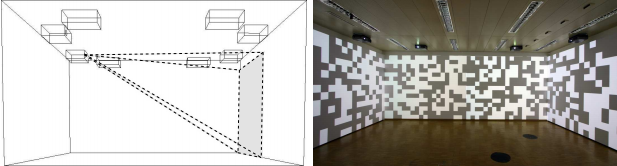
\includegraphics[width=\textwidth]{../figures/Murallas.png}
\end{figure}}

\only<2>{Infrarrojo

\begin{itemize}

\item Transmisor infrarrojo con un identificador único.

\item Receptores son colocados en lugares dentro del recinto, los cuales pueden detectar este identificador único y comunicar a un software especializado.

\item No se afecta por interferencia electromagnética. Costoso y complejo.
\end{itemize}
}

\only<3>{Tecnologías basadas en Sonido

\begin{figure}
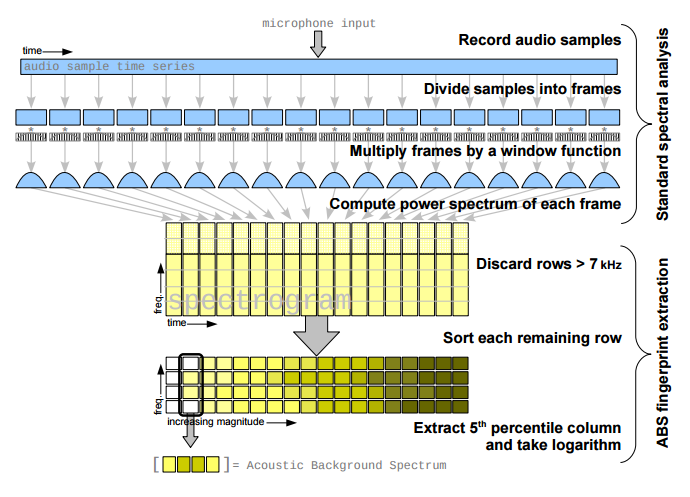
\includegraphics[width=0.8\textwidth]{../figures/abs.png}
\end{figure}
}

\only<4>{RFID

\begin{itemize}
\item La localización mediante RFID puede categorizarse en dos tipos, los cuales son localización del lector y localización de tags.

\item Costoso y no escalable.

\item Poco alcance, sin embargo, no necesita línea de visión directa.
\end{itemize}
}

\only<5>{Tecnologías Inalámbricas

\begin{block}{Received Signal Strength Indicator}
RSSI es una escala de referencia para medir el nivel de potencia de la fuerza de la señal recibida por el receptor. Se mide en dBm donde 0 RSSI indica señal ideal y valores más negativos indican mayor perdida. 
\end{block}

\begin{block}{Tx Power}
Es la potencia de salida o fuerza de la señal que el emisor produce durante el tiempo de transmisión. A mayor Tx Power, más estable es la señal, pero más energía se consume.
\end{block}
}

\only<6> { Comparativa de tecnologías

\begin{figure}
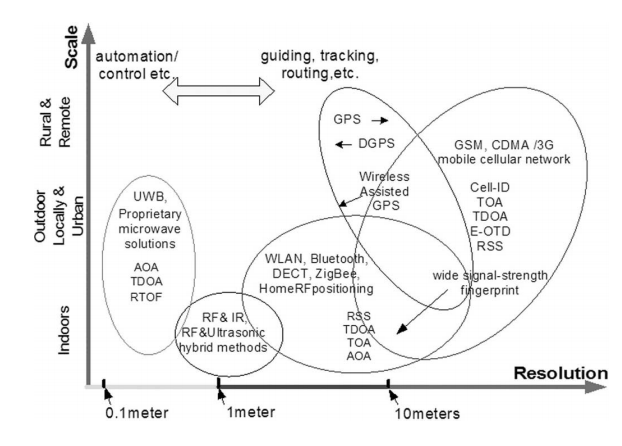
\includegraphics[width=0.8\textwidth]{../figures/comparativa.png}
\end{figure}

}


\end{frame}

%------------------------------------------------
\subsection{Técnicas  matemáticas Wireless para localización indoor}
\begin{frame}
\frametitle{Proximidad}

\begin{itemize}

\item Es el método más simple, y se basa en determinar una posición simbólica y aproximada de la posición del usuario.

\item Antenas o emisores de ondas de radio. Según la señal más fuerte detectada por el usuario, es donde se localiza en el sistema.

\item Ampliamente usado en redes celulares, ya que permite determinar la posición de un dispositivo con una precisión de 50-200 metros, sin embargo, no es buena en espacios reducidos. GSM, Infrarrojo, Cell-ID.
\end{itemize}


\end{frame}

%------------------------------------------------

\begin{frame}
\frametitle{Triangulación}

\begin{figure}
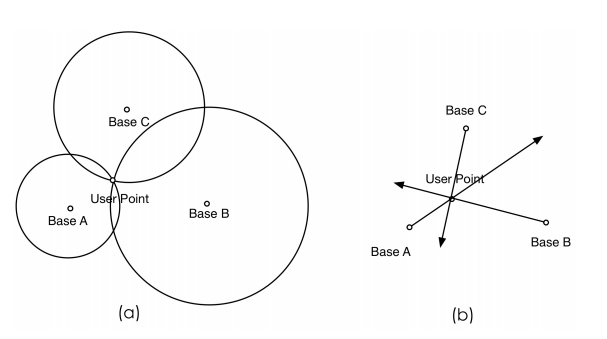
\includegraphics[width=\linewidth]{../figures/triangulacion.png}
\end{figure}

\end{frame}

%------------------------------------------------

\begin{frame}
\frametitle{Fingerprint}

\begin{figure}
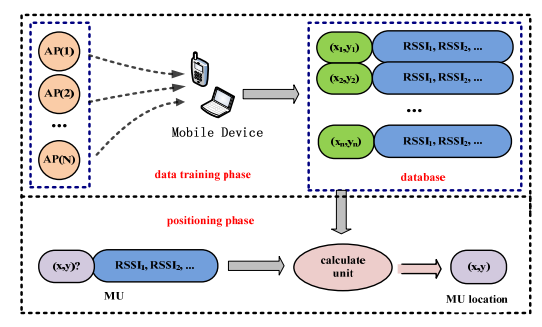
\includegraphics[width=.8\linewidth]{../figures/finger.png}
\end{figure}

\end{frame}


%------------------------------------------------
\section{Propuesta de solución}
%------------------------------------------------

\begin{frame}
\frametitle{Propuesta}

\begin{itemize}
\item Establecer un marco de trabajo para la recolección, entrenamiento y clasificación de algoritmos de machine learning utilizando Bluetooth Low Energy.\\

\pause

\item Comparación de diferentes clasificadores.\\

\pause
\item Utilizar técnicas de reducción de dimensionalidad.\\
\pause

\item Utilizar modelos sin necesidad de conexión a internet.
\end{itemize}

\end{frame}


%------------------------------------------------
\subsection{Consideraciones Previas}

\begin{frame}
\frametitle{Beacons}

\begin{columns}[t] % The "c" option specifies centered vertical alignment while the "t" option is used for top vertical alignment

\column{.5\textwidth} % Left column and width

\begin{itemize}
\item \onslide<1->{La transmisión corresponde a un ID único que está presente en cada Beacon y que no se repite, como una dirección MAC o un UUID.}

\item \onslide<2->{Auge del Internet de las cosas.}

\item \onslide<3->{Habitualmente los Beacons soportan ambos protocolos existentes, es decir IBeacon y Eddystone.}

\end{itemize}

\column{.5\textwidth} % Right column and width
\begin{figure}
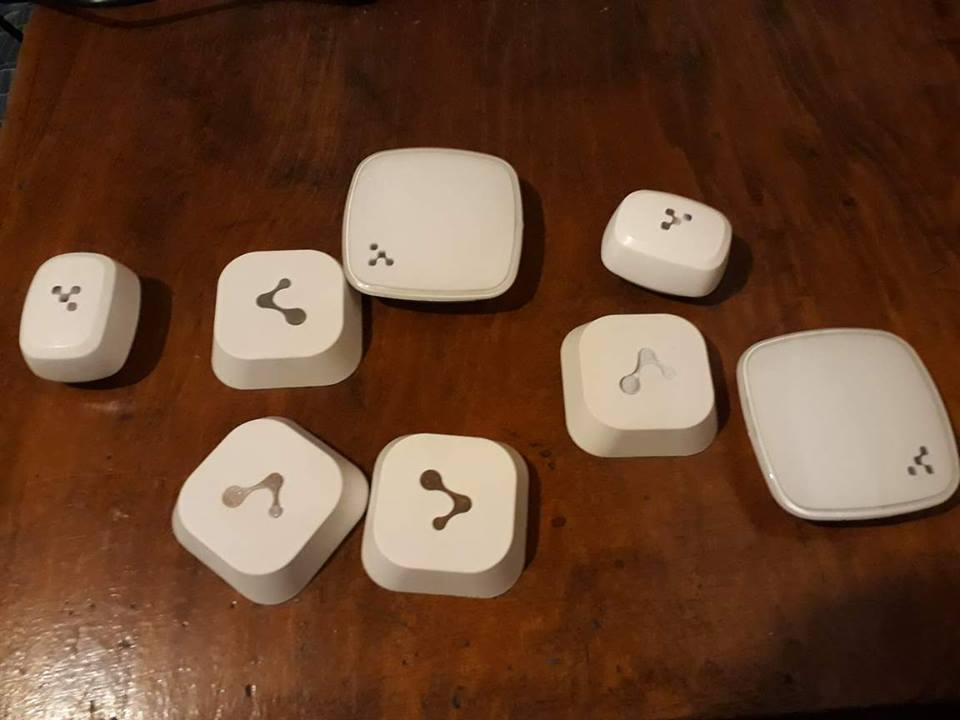
\includegraphics[width=\textwidth]{../figures/beacons_all.jpg}

\end{figure}

\end{columns}

\end{frame}

%------------------------------------------------
\begin{frame}
\frametitle{Beacons - Valores esperados}

\begin{table}[ht!]
\centering
\resizebox{\columnwidth}{!}{
\begin{tabular}{|c|c|c|}
Parámetro                   & Kontakt.io                      & Estimote                             \\ \hline
Duración de la batería      & Hasta 4 años                    & Hasta 2 años                         \\ \hline
Rango                       & 70m                             & 70m                                  \\ \hline
Procesador                  & 32-bit ARM® Cortex™ M0 CPU core & ARM® Cortex®-M4 32-bit processor FPU \\ \hline
Sensibilidad                & -93dBm                          & -96 dBm                              \\ \hline
Velocidades                 & 250kBs, 1Mbs, y 2Mbs            & 1 Mbps (2 Mbps soportado)            \\ \hline
Memoria                     & 256KB flash 16KB RAM            & 512 kB Flash memory 64 kB RAM memory \\ \hline
Transmission power          & -30dBm a 4dBm                  & -20dBm a +4 dBm                        \\ \hline
Batería                     & 2 x 1.000mAh CR2477             & 1 x CR2477 – 3.0V                    \\ \hline
Bluetooth                   & Bluetooth® 4.2 LE standard      & Bluetooth® 4.2 LE standard           \\ \hline
Espesor                     & 15mm                            & 17mm                                 \\ \hline
Peso                        & 35 gr                           & 30 gr                                \\ \hline
Paquete IBeacon y Eddystone & 1 a la vez                      & 1 a la vez                           \\ \hline
Paquetes adicionales        & telemetría                      & telemetría                           \\ \hline
Sensores adicionales        & Temperatura                     & movimiento, temperatura              \\ \hline
Batería reemplazable        & Si                              & Si                                   \\ \hline
Numero de Beacons           & 3                               & 3                                    \\ \hline
Precio                      & 60 USD                          & 59 USD                               \\ \hline
\end{tabular}
}
\end{table}
\end{frame}

%------------------------------------------------

\begin{frame}
\frametitle{Estabilidad de la señal Bluetooth}

\begin{itemize}
\item Se realiza prueba para comprobar cómo afecta las interferencias a la señal Bluetooth.

\end{itemize}

\begin{figure}
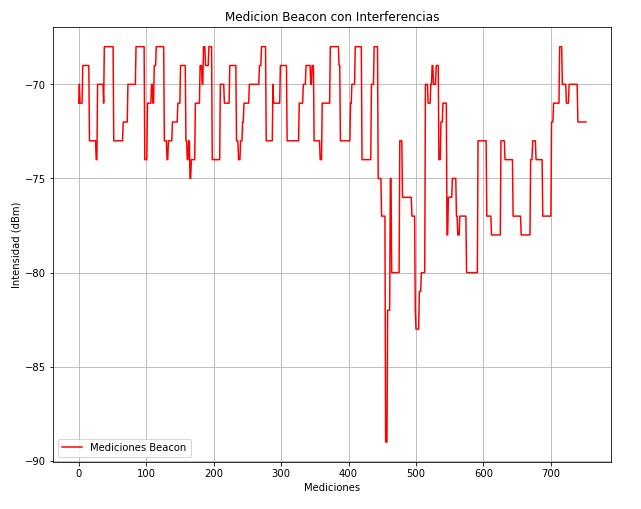
\includegraphics[width=.7\textheight]{../figures/mediciones_beacon_interferencia.jpg}
\end{figure}

\end{frame}

%------------------------------------------------

\begin{frame}
\frametitle{Algoritmos de \textit{Machine Learning}}

\begin{columns}[t] % The "c" option specifies centered vertical alignment while the "t" option is used for top vertical alignment

\column{.33\textwidth}

\begin{center}k-NN\end{center}

\begin{figure}
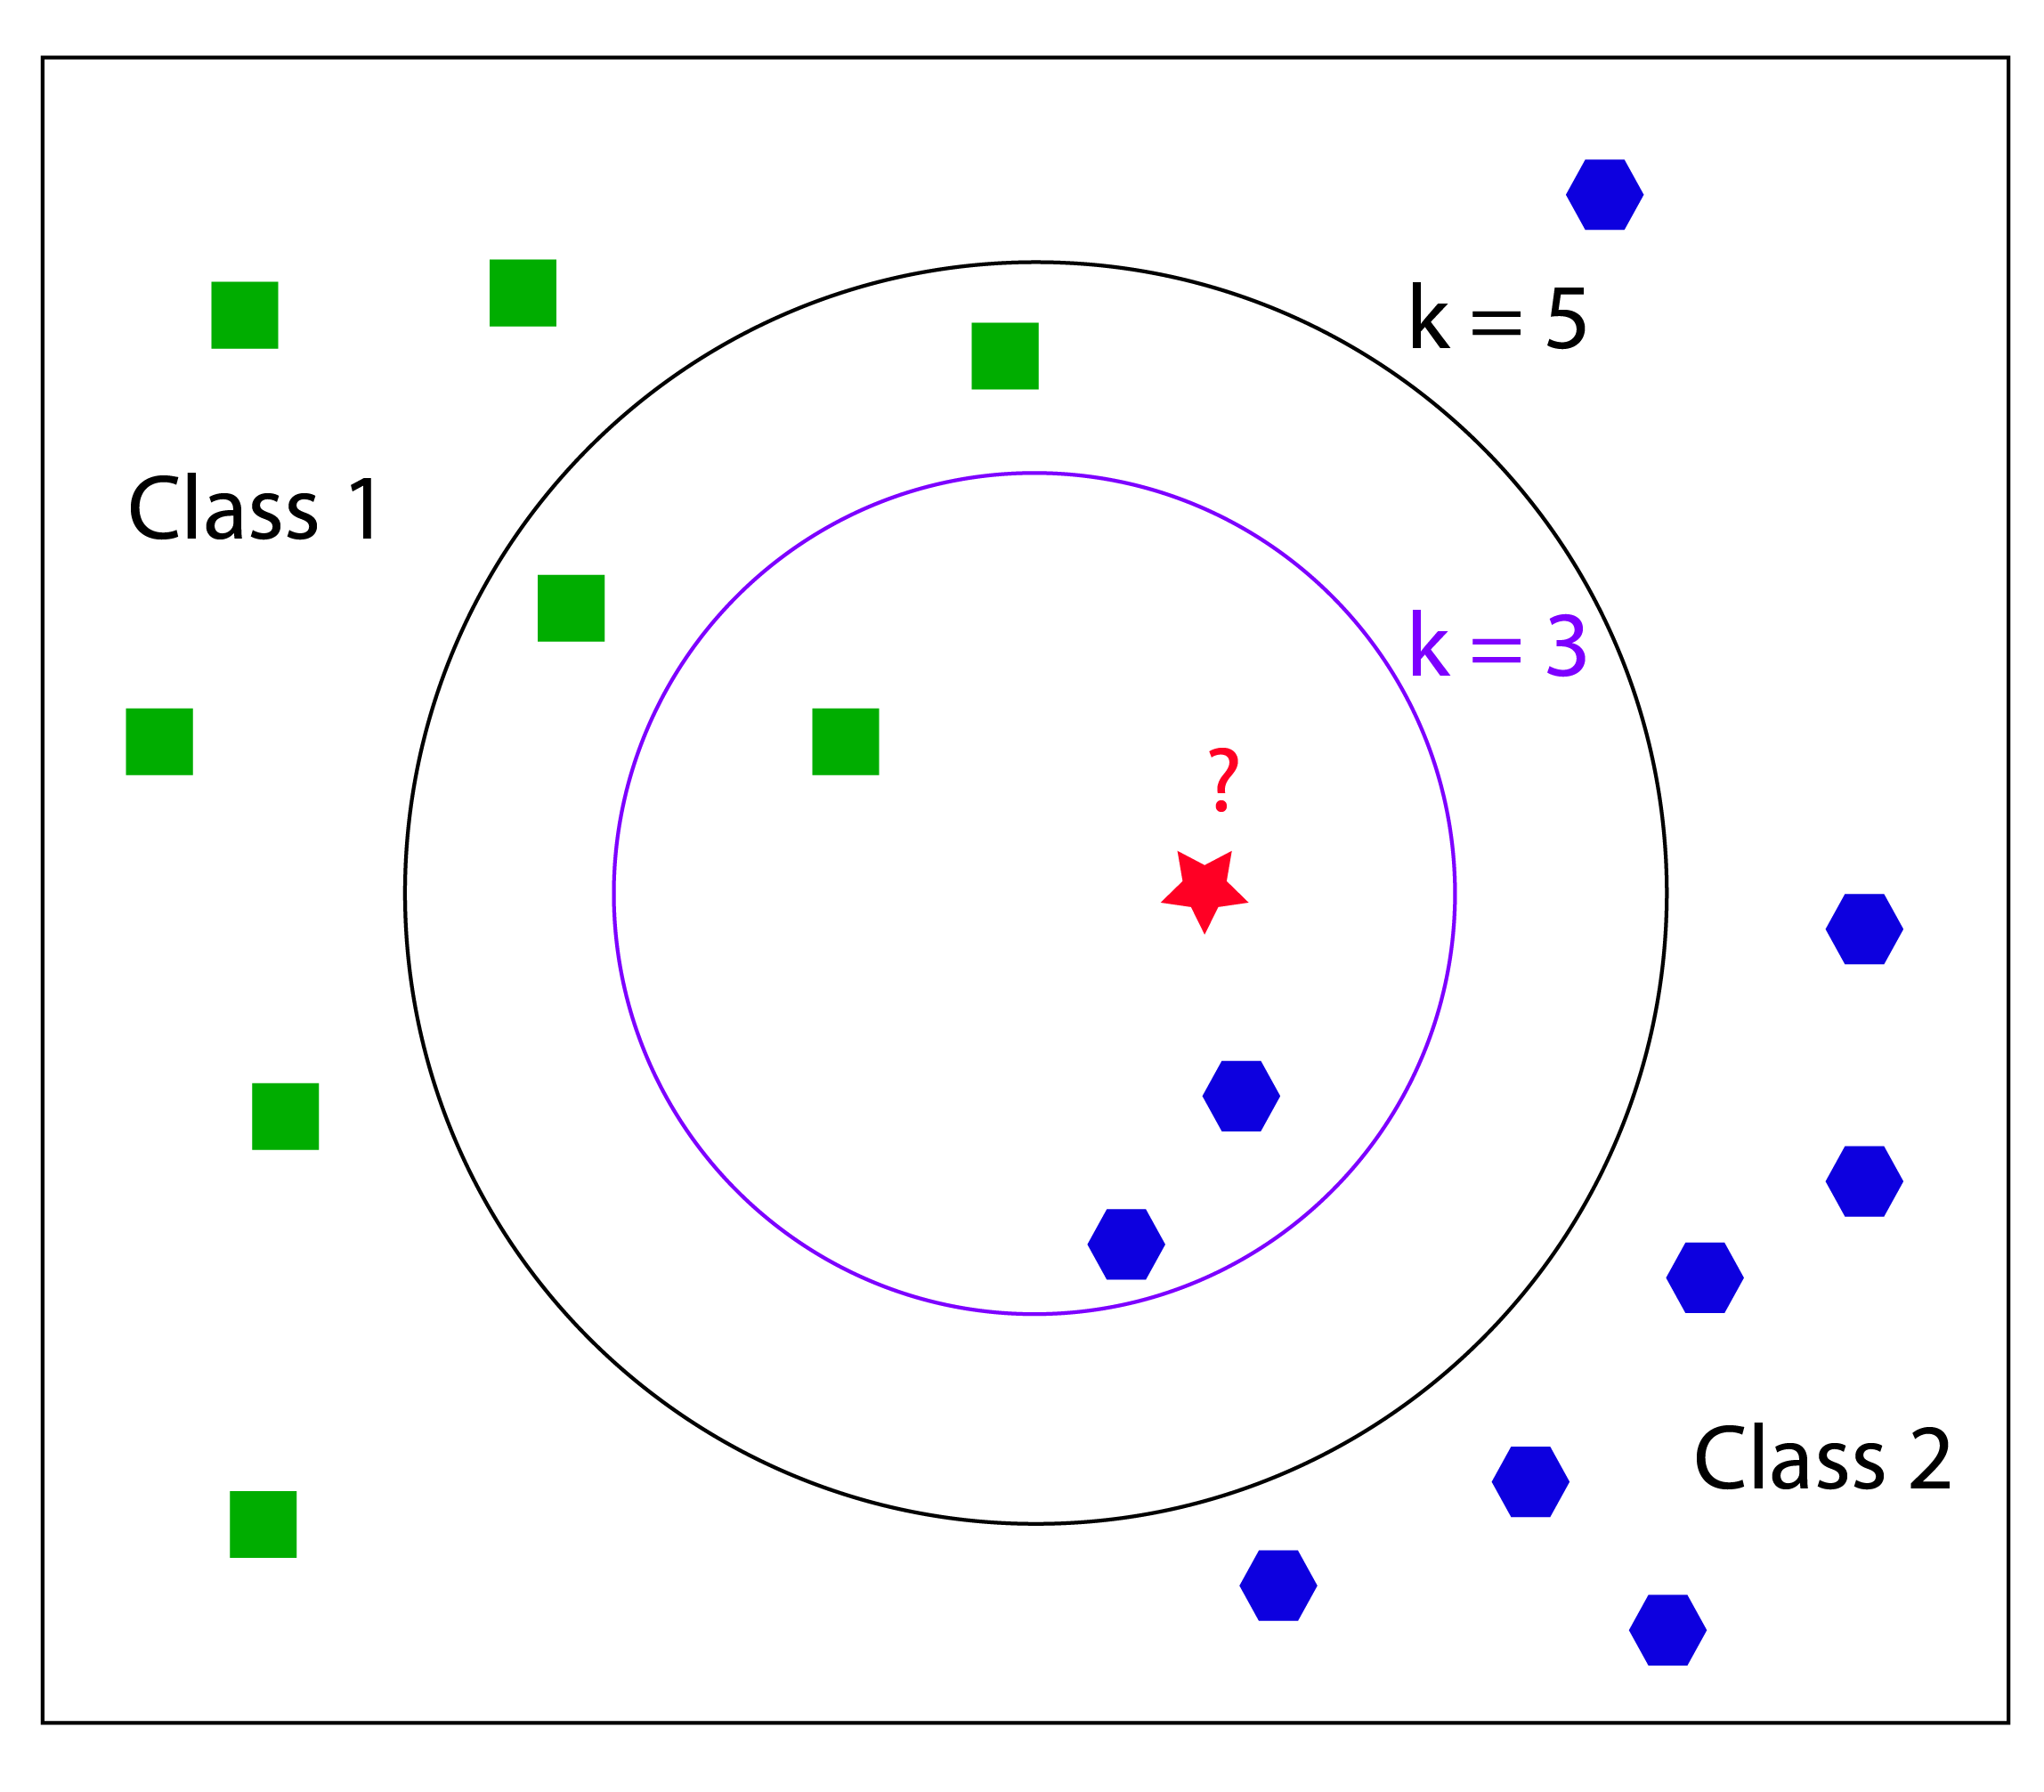
\includegraphics[width=\textwidth]{../figures/knn.png}
\end{figure}

\pause

\column{.33\textwidth}

\begin{center}SVM\end{center}

\begin{figure}
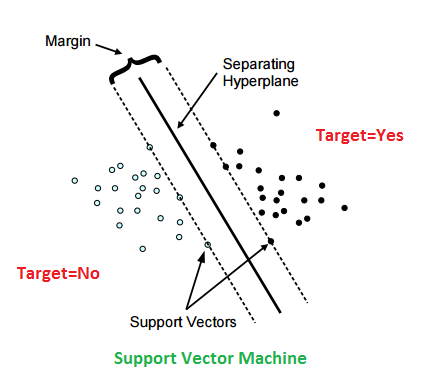
\includegraphics[width=\textwidth]{../figures/SVM-Planes.png}
\end{figure}

\pause

\column{.33\textwidth}

\begin{center}Neural Networks\end{center}

\begin{figure}
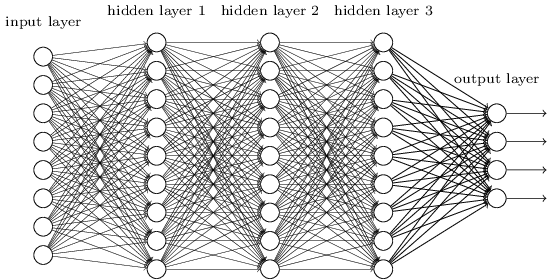
\includegraphics[width=\textwidth]{../figures/deep.png}
\end{figure}

\end{columns}

\end{frame}

%------------------------------------------------
\subsection{Descripción del \textit{framework} de posicionamiento}
\begin{frame}
\frametitle{Descripción del \textit{framework} de posicionamiento}

\begin{itemize}

\item Establecer un marco de trabajo.

\pause

\item Se utiliza la técnica de Fingerprint discutida en el estado del arte, mediante la utilización de un mapa de señales, también denominado \textit{radiomap}.

\pause

\item Utilizar dispositivos Bluetooth Low Energy, lo cuales realizan la función de access point(AP) y que serán los responsables de emitir la señal RSSI. Luego, el procedimiento se divide en las dos clásicas etapas de Fingerprint, es decir, fase \textit{offline} y fase \textit{online}.
\end{itemize}


\end{frame}

%------------------------------------------------


\begin{frame}
\frametitle{Fase Offline}

\begin{itemize}
\item Crear un tipo de aplicación que sea capaz de recolectar los vectores RSSI.

\pause

\item El periodo y frecuencia de los datos se debe determinar experimentalmente. Para ello, cada medición a colectar representa un punto en el espacio $2-dimensional$.

\pause

\item Para generar la grilla, es necesario tener la posición exacta, que corresponde a la etiqueta de cada punto.

\pause

\item Con los datos registrados, se debe crear la base de datos que almacenara estos Fingerprints, ya que desde ahí es posible analizar los datos y mantener su persistencia
\end{itemize}


\end{frame}

%------------------------------------------------

\begin{frame}
\frametitle{Fase Offline}

\begin{figure}
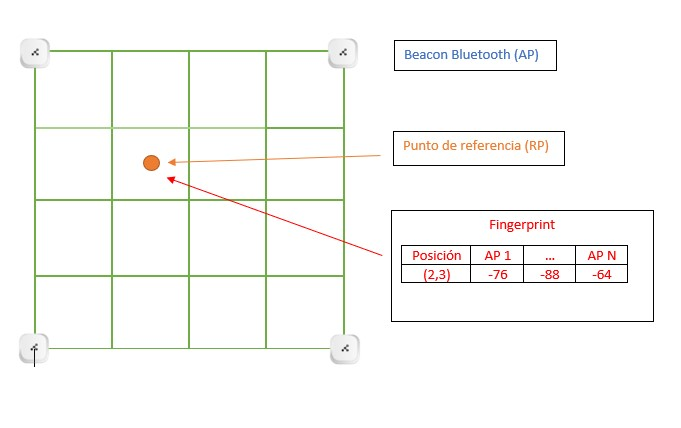
\includegraphics[width=\textwidth]{../figures/fingerprints.jpg}
\end{figure}

\end{frame}

%------------------------------------------------

\begin{frame}
\frametitle{Reducción de dimensionalidad}

\begin{itemize}

\item Esto no ha sido mayormente explorado en la literatura

\pause
\item Existe correlación espacial lineal de las señales adyacentes. PCA ayuda a eliminar esta correlación.
\pause

\item Los métodos de extracción de características pueden ayudar a agilizar la fase de entrenamiento, ya que este proceso es lento.

\pause

\item Descubrir atributos en un espacio no correlacionado. Transformación lineal del vector RSSI.

\end{itemize}

\end{frame}

%-------------------------------------------------

\begin{frame}
\frametitle{Entrenamiento de algoritmos}

\begin{itemize}

\item Entrenar técnicas de máquinas de aprendizaje.

\pause
\item Posteriormente, se seleccionan los mejores algoritmos y luego son implementados.
\pause

\item \textbf{¿Implementación en cliente o servidor?}

\end{itemize}

\end{frame}

%-------------------------------------------------

\begin{frame}
\frametitle{Fase Online}

\begin{itemize}

\item Para la fase online se reconocen dos etapas principales.

\begin{enumerate}
\pause
\item Colectar un vector de señales RSSI en la posición actual del usuario.
\pause
\item Proveer este vector de entrada a los algoritmos de aprendizaje supervisado ya entrenados.
\end{enumerate}

\pause
\item Una vez que los algoritmos de clasificación proveen el resultado de la posición física, entonces la misma aplicación de la fase offline, es utilizada para mostrar en un mapa de tiempo real la localización actual de usuario.

\pause

\item Para realizar esta tarea se deben tener en cuenta las normalizaciones realizadas y aplicar correctamente la transformación PCA.


\end{itemize}
\end{frame}


%-------------------------------------------------

\begin{frame}
\frametitle{Proceso de desarrollo}

\begin{figure}
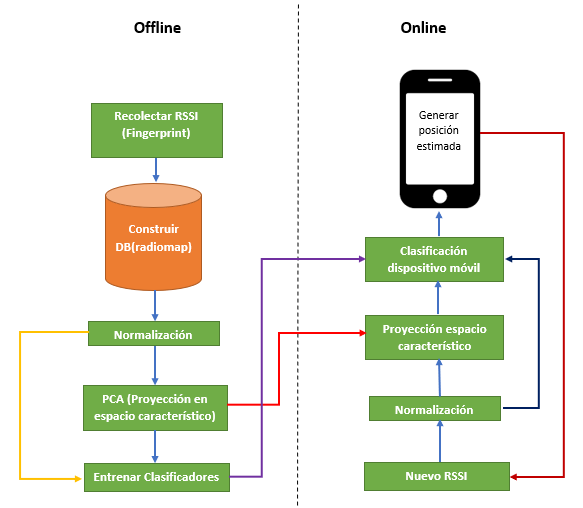
\includegraphics[width=0.7\textwidth]{../figures/propuesta_memoria.png}
\end{figure}


\end{frame}

%-------------------------------------------------
\section{Experimentación}
%-------------------------------------------------

\subsection{Implementación}

\begin{frame}
\frametitle{Beacons y configuración}

\begin{columns}[t] % The "c" option specifies centered vertical alignment while the "t" option is used for top vertical alignment

\column{.5\textwidth} % Left column and width
\begin{figure}
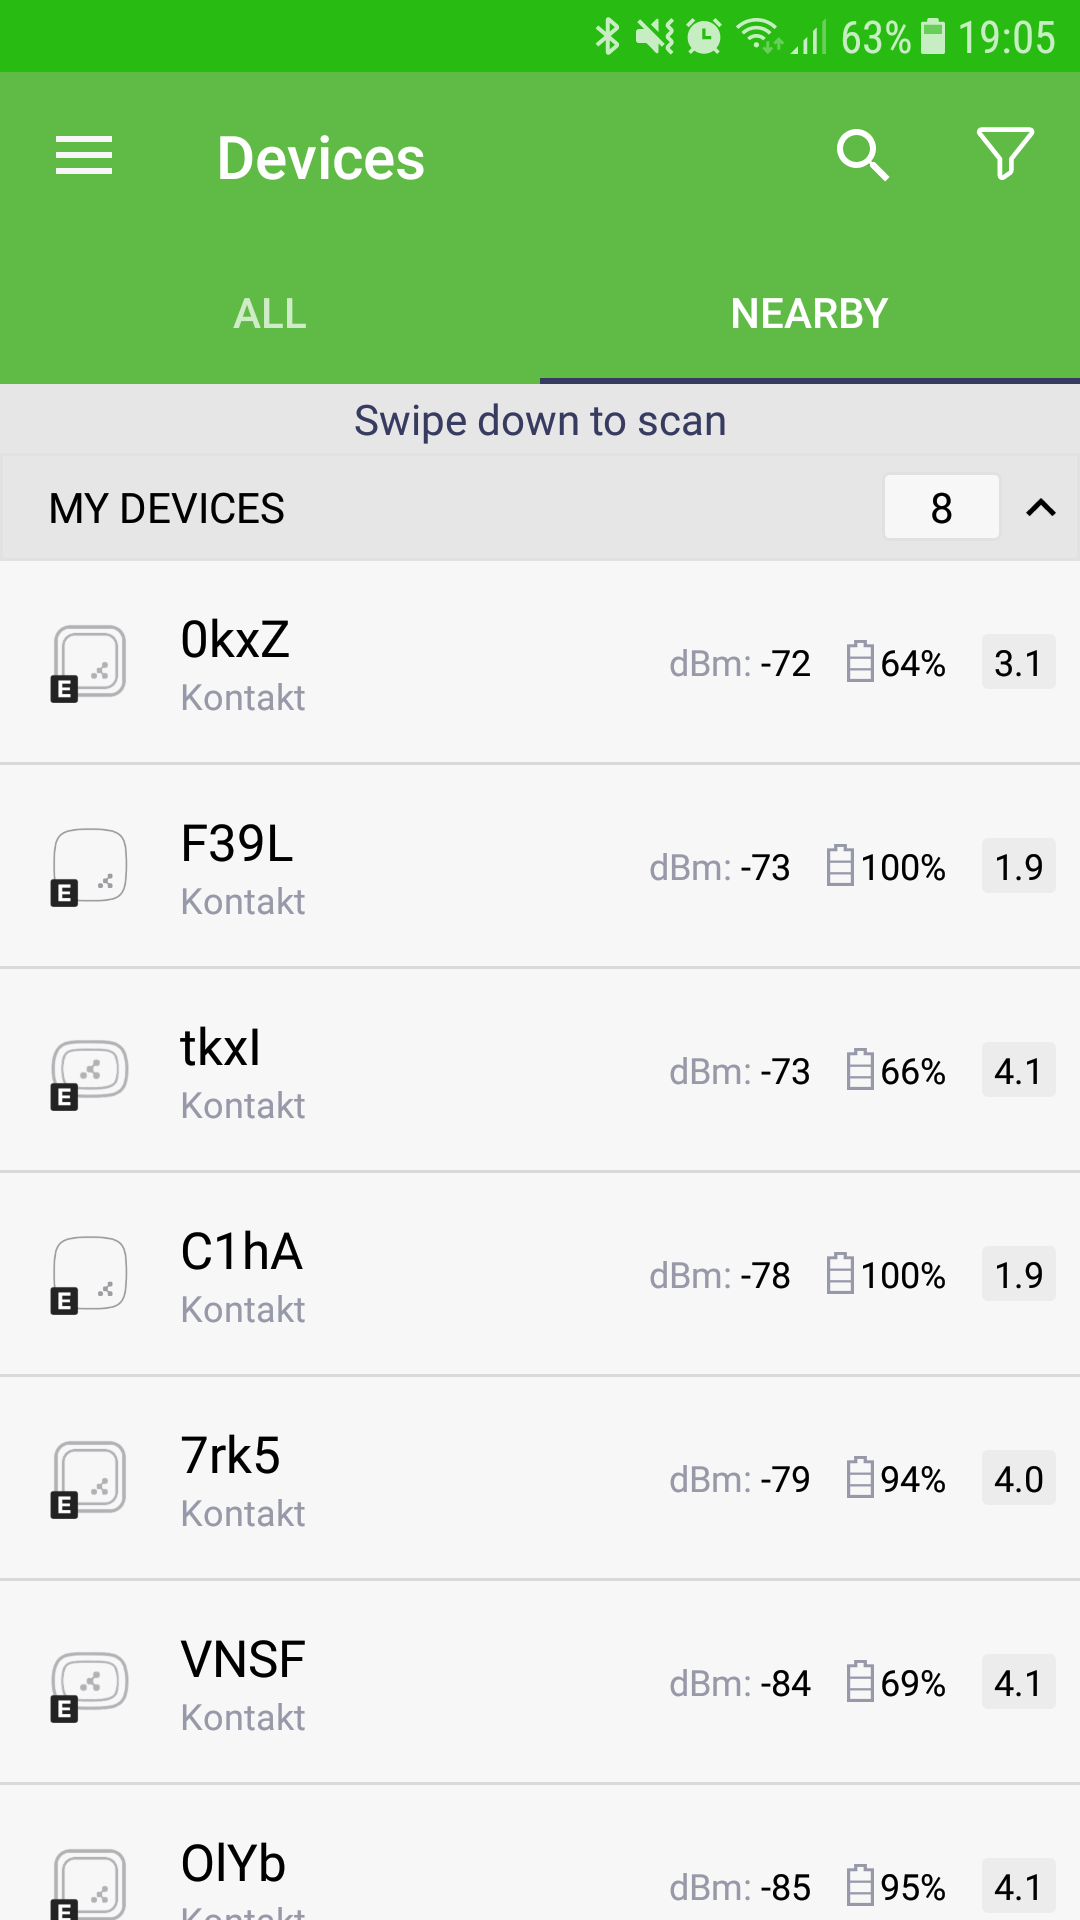
\includegraphics[width=0.6\textwidth]{../figures/kontaktapp1.png}
\end{figure}

\column{.5\textwidth} % Right column and width
\begin{figure}
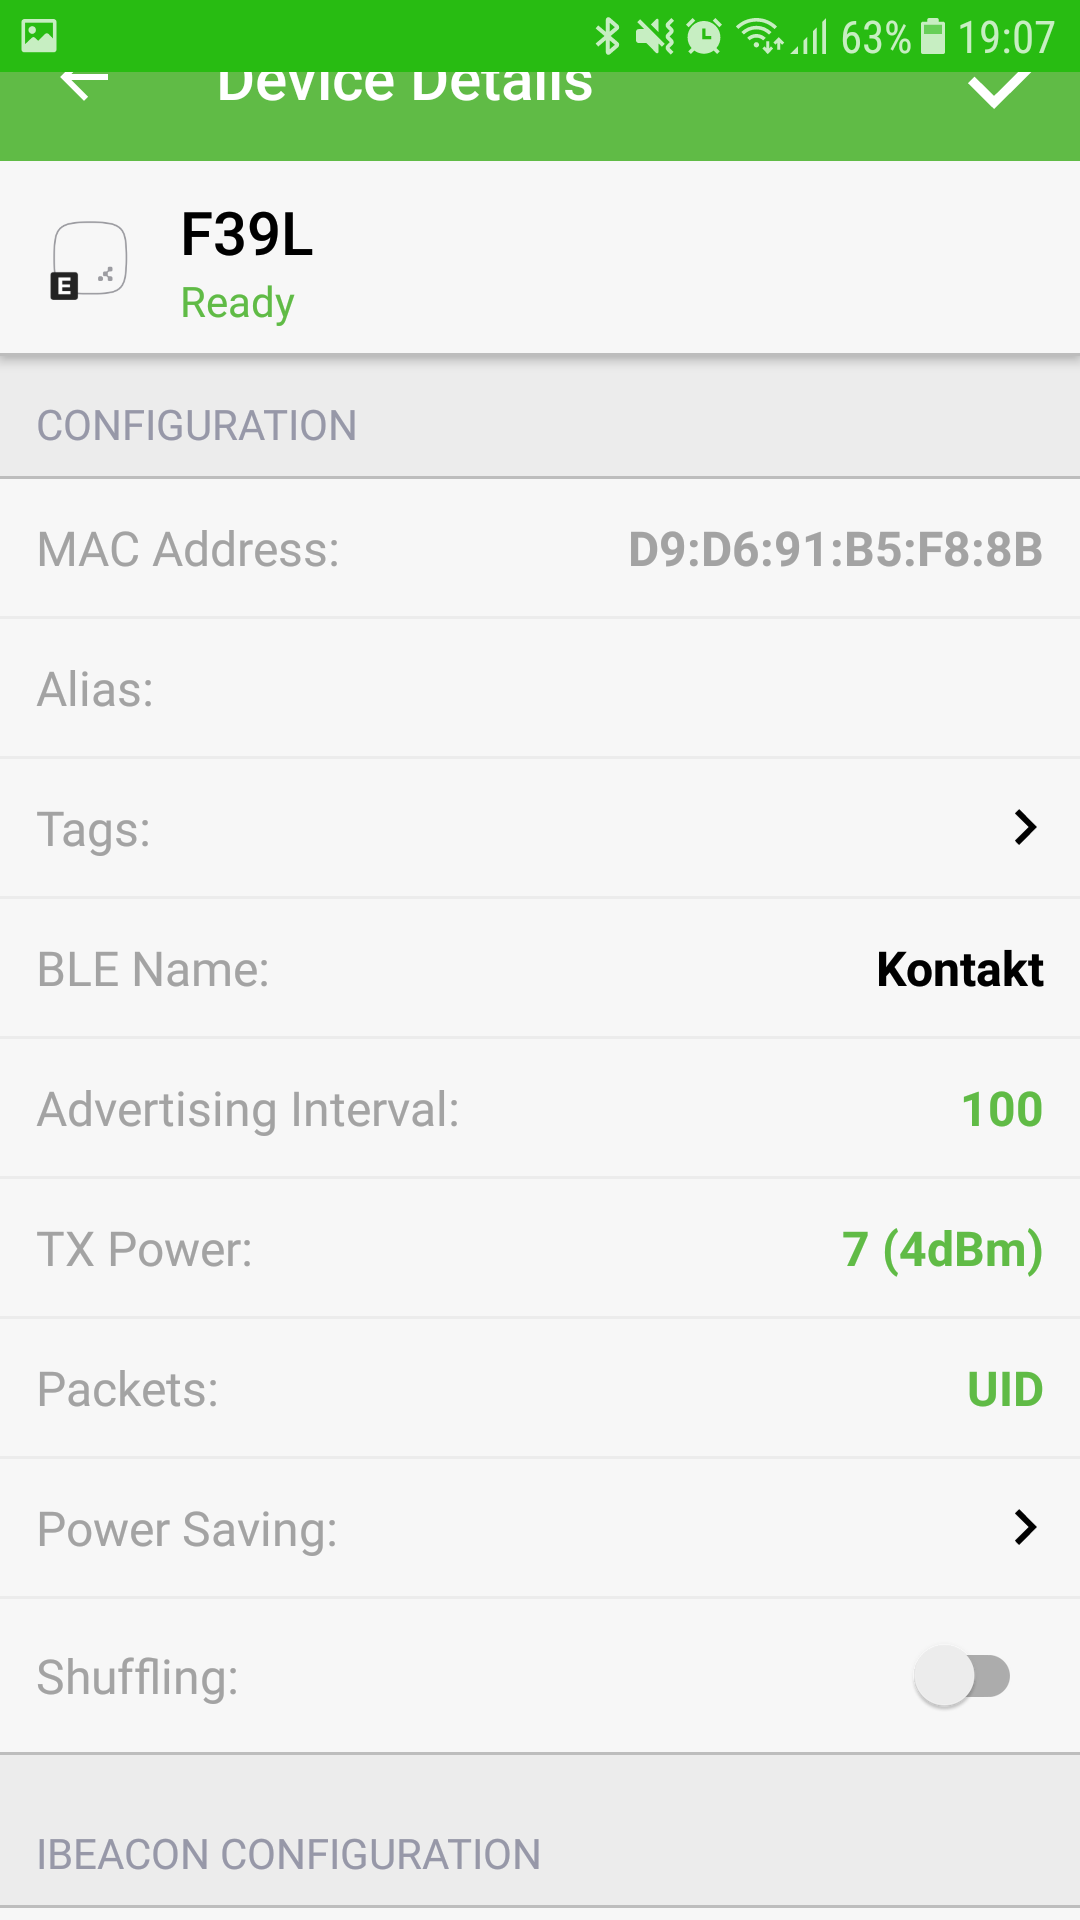
\includegraphics[width=0.6\textwidth]{../figures/kontaktapp2.png}
\end{figure}

\end{columns}
\end{frame}
%------------------------------------------------

\begin{frame}
\frametitle{Lugar de experimentación}

Estacionamiento subterráneo de la universidad Técnica Federico Santa María, Campus San Joaquín.

\begin{columns}[t] % The "c" option specifies centered vertical alignment while the "t" option is used for top vertical alignment

\column{.5\textwidth} % Left column and width
\begin{figure}
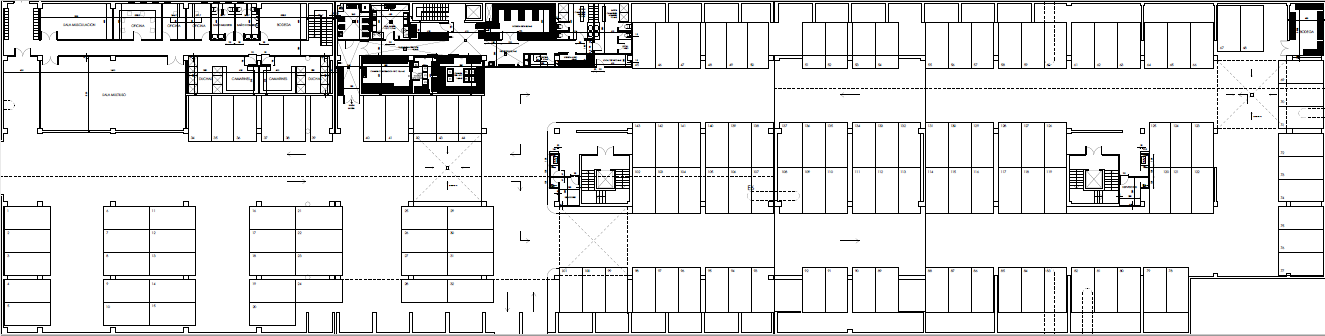
\includegraphics[width=\textwidth]{../figures/estSubterraneo.png}
\end{figure}

\column{.5\textwidth} % Right column and width
\begin{figure}
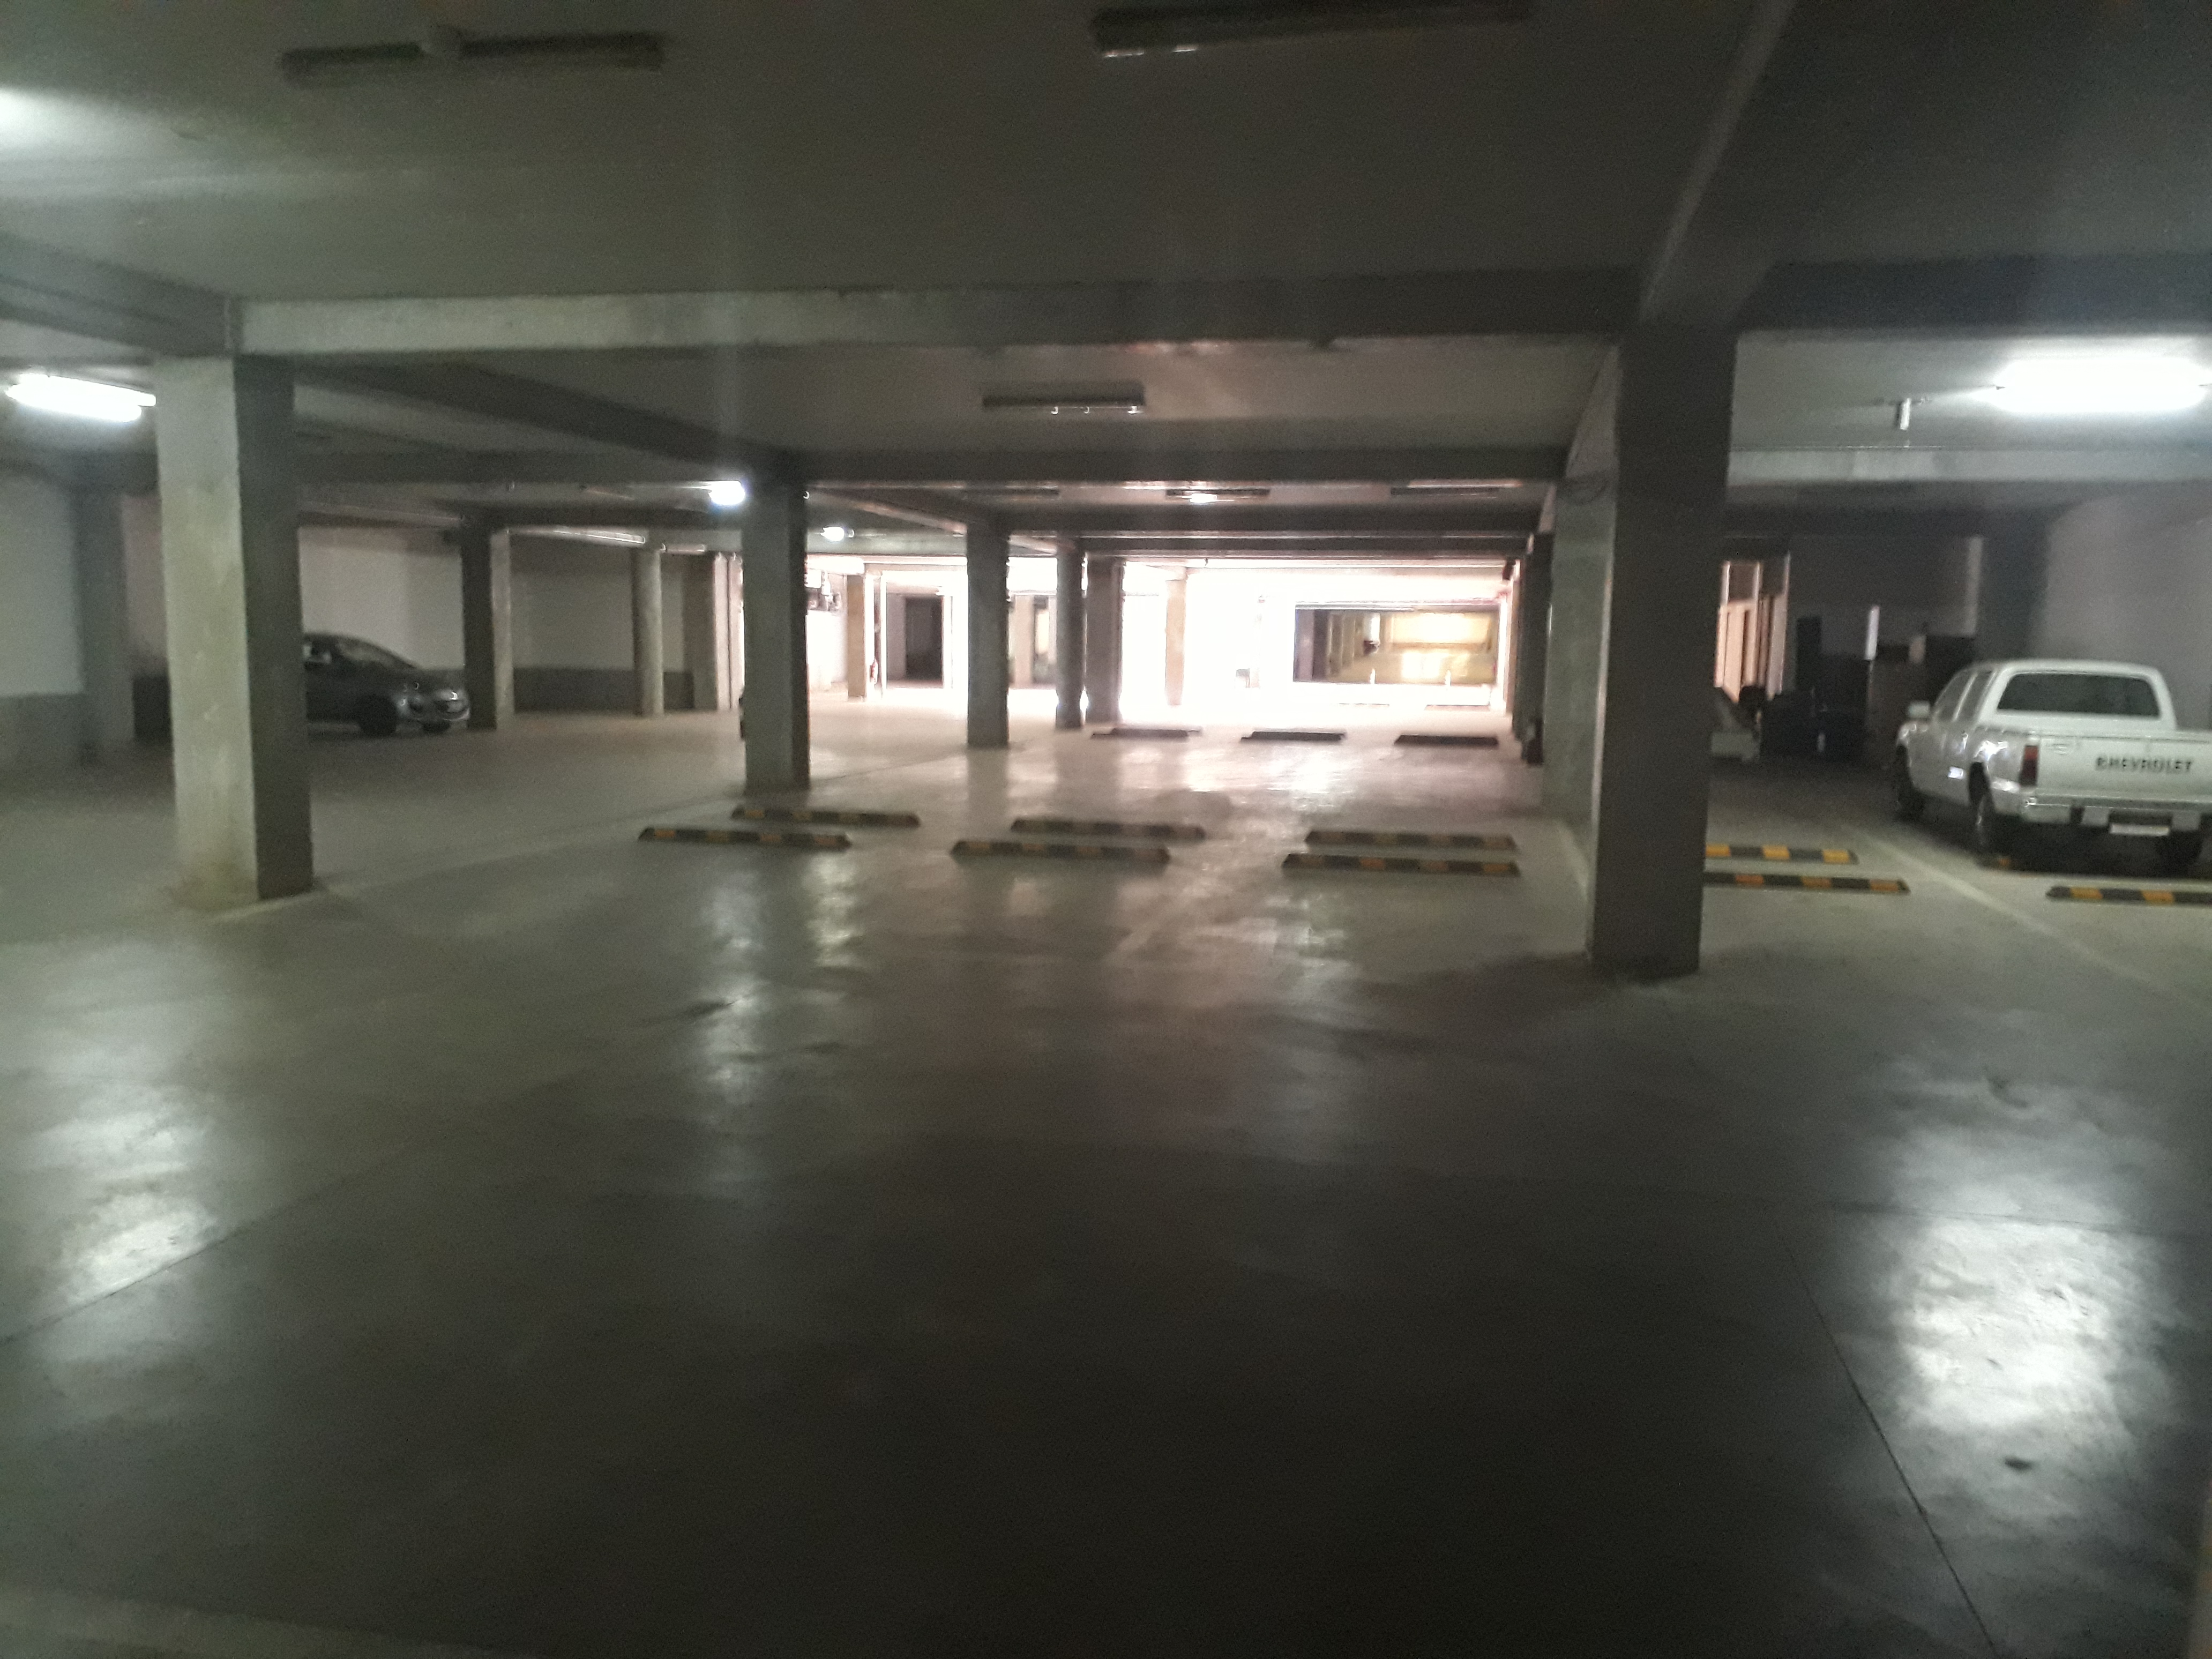
\includegraphics[width=\textwidth]{../figures/estReal.jpg}
\end{figure}

\end{columns}

\end{frame}

%------------------------------------------------

\begin{frame}
\frametitle{Software Utilizado}

\begin{itemize}
\item Aplicación Android:
	\begin{enumerate}[1]
\onslide<1->{\item Mostrar el plano del lugar de experimentación.}

\onslide<2->{\item Permitir la adición de nuevos dispositivos Beacons.}

\onslide<3->{\item Permitir la captura de datos, es decir, los nuevos Fingerprints. }

\onslide<4->{\item Modificar los valores de intervalo y el número de mediciones en cada punto, el cual puede también definirse en periodo de tiempo.}

\onslide<5->{\item Tener una base de datos \textit{SQLite}.}

\onslide<6->{\item Para la etapa online, debe permitir seleccionar el algoritmo a utilizar y mostrar en tiempo real la posición del usuario.}

\end{enumerate}

\onslide<7->{\item Scikit-learn}

\onslide<8->{\item Tensorflow}

\end{itemize}

\end{frame}

%------------------------------------------------

\begin{frame}
\frametitle{Recolección de Fingerprints}

\begin{columns}[t] % The "c" option specifies centered vertical alignment while the "t" option is used for top vertical alignment

\column{.7\textwidth} % Left column and width

\begin{itemize}
\onslide<1->{\item Samsung Galaxy J7 Prime,CPU Octa-core 1.6 GHz Cortex-A53, una GPU Mali-T830 MP1, 3GB de memoria ram interna y el tipo de Bluetooth corresponde a 4.1 LE}

\onslide<2->{\item 8 beacons en un área reducida del estacionamiento y ubicar cada Beacon a una distancia de 16 metros a sus vecinos adyacentes. 16 x 44 metros ($704m^2$). }


\onslide<3->{\item Grilla para los puntos de referencia de 4 metros por 4 metros, 44 en total. }
\end{itemize}

\column{.5\textwidth} % Right column and width
\onslide<1->{\begin{figure}
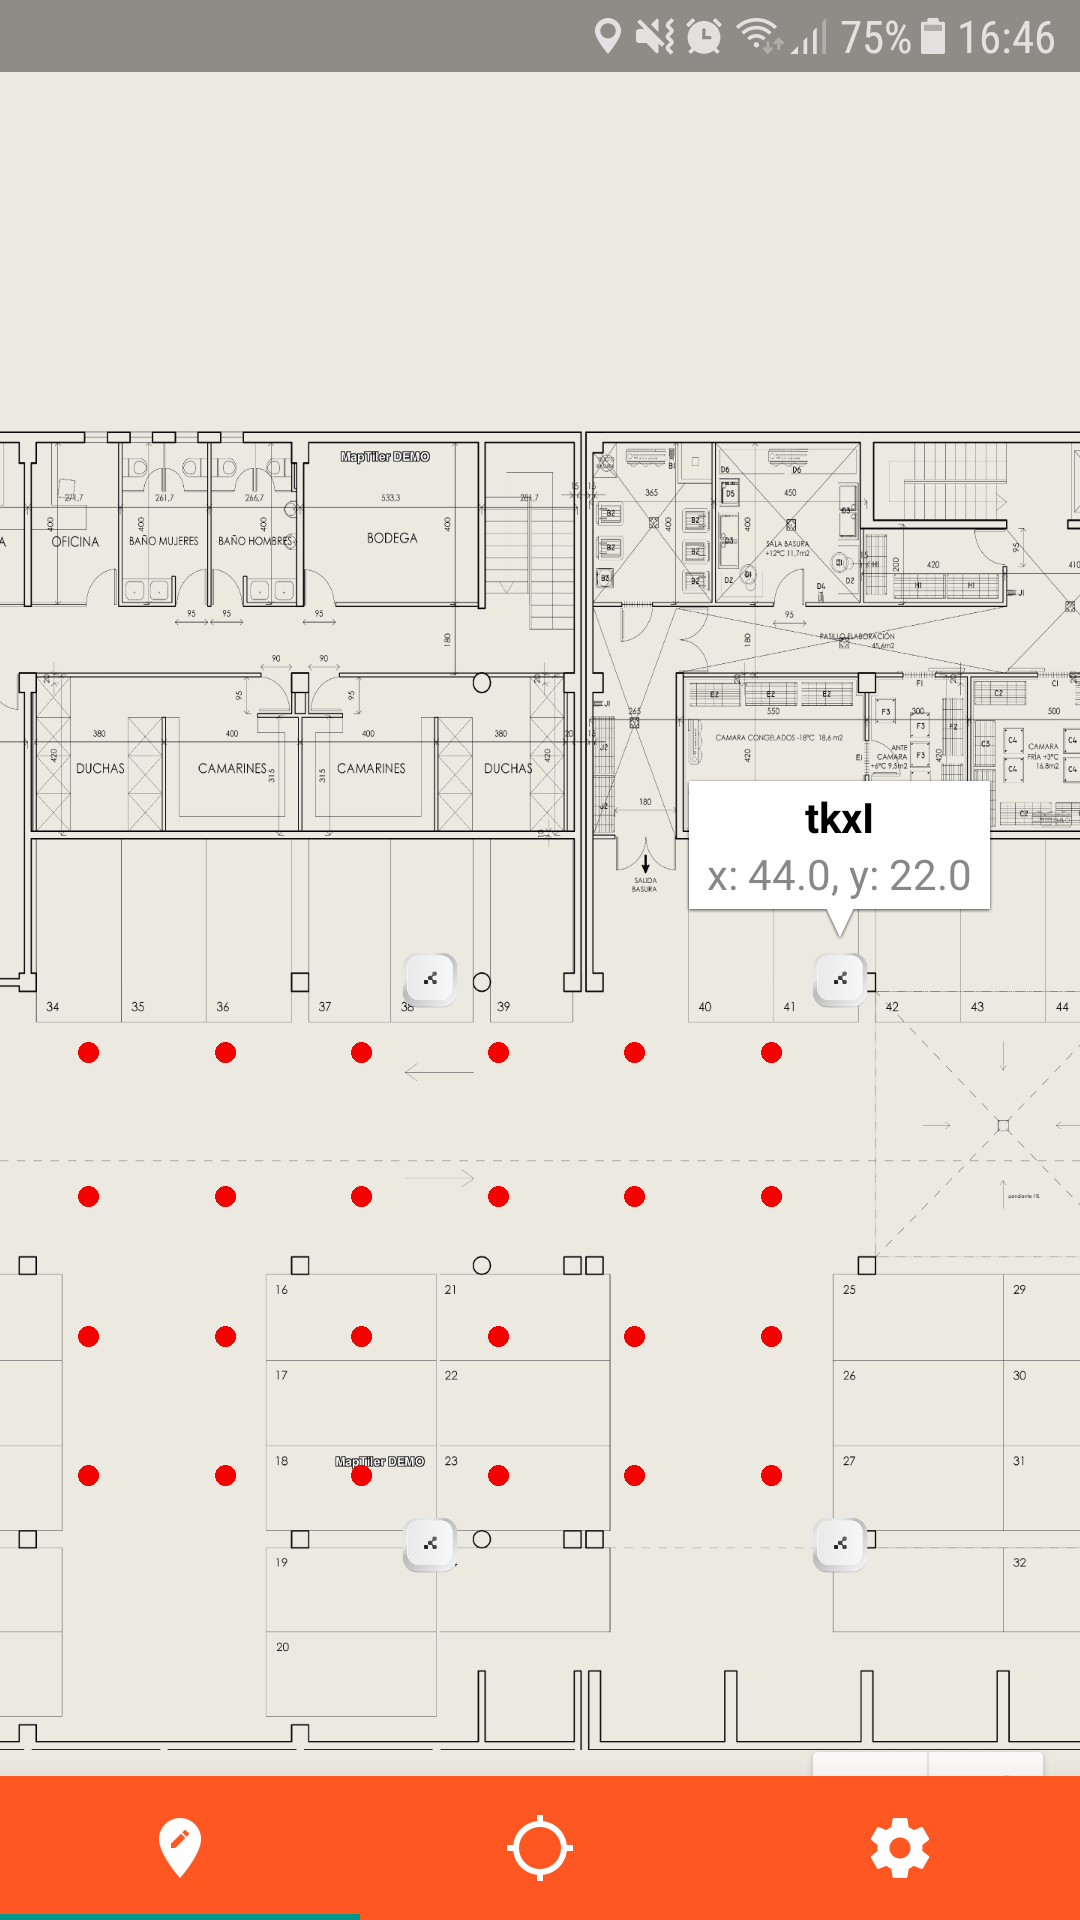
\includegraphics[width=0.65\textwidth]{../figures/deployBeacons.png}
\end{figure}
}

\end{columns}

\end{frame}

%------------------------------------------------

\begin{frame}
\frametitle{Recolección de Fingerprints}

\begin{columns}[t] % The "c" option specifies centered vertical alignment while the "t" option is used for top vertical alignment

\column{.7\textwidth} % Left column and width

\begin{itemize}
\onslide<1->{\item 3000 mediciones por posición. Se decide inspeccionar y recolectar datos a través de diferentes días.}

\onslide<2->{\item Se seleccionan 150 mediciones por punto de la grilla, para tener menor información repetida y no sobre muestrear la base de datos.}


\onslide<3->{\item Se obtiene una base de datos \textit{SQLite} con Figerprints, la cual presenta 6600 registros}

\onslide<4->{\item Clases X e Y son las posiciones asociadas a cada coordenada.}
\end{itemize}

\column{.5\textwidth} % Right column and width
\onslide<1->{\begin{figure}
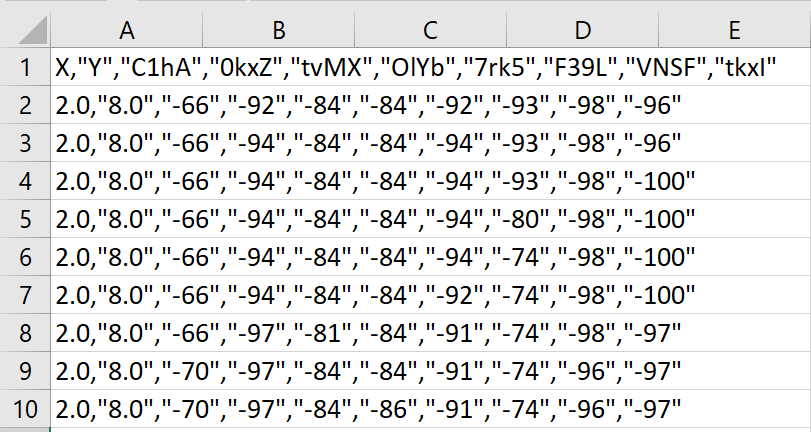
\includegraphics[width=\textwidth]{../figures/ejemplo_csv.png}
\end{figure}
}

\end{columns}

\end{frame}

%-------------------------------------------------
\begin{frame}
\frametitle{Entrenamiento de clasificadores}

\begin{columns}[t] 
\column{.5\textwidth} % Left column and width

\only<1>{\begin{figure}
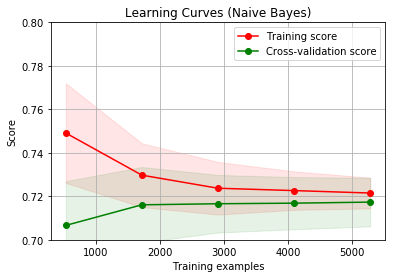
\includegraphics[width=\textwidth]{../figures/NB.png}
\end{figure}}

\only<2>{\begin{figure}
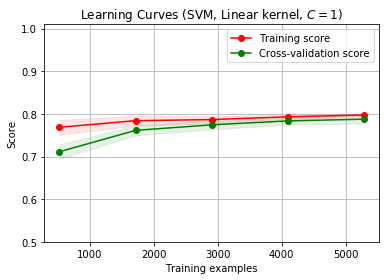
\includegraphics[width=\textwidth]{../figures/SVM-Lineal.png}
\end{figure}}

\only<3>{\begin{figure}
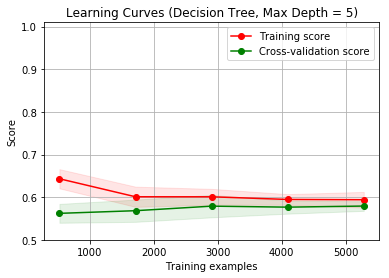
\includegraphics[width=\textwidth]{../figures/decision-tree.png}
\end{figure}}

\only<4>{\begin{figure}
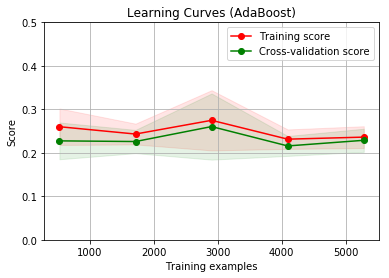
\includegraphics[width=\textwidth]{../figures/adaboost.png}
\end{figure}}

\column{.5\textwidth} % Right column and width
\only<1>{\begin{figure}
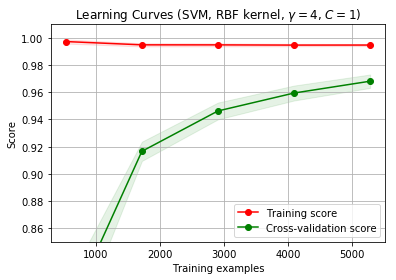
\includegraphics[width=\textwidth]{../figures/SVM-RBF.png}
\end{figure}}

\only<2>{\begin{figure}
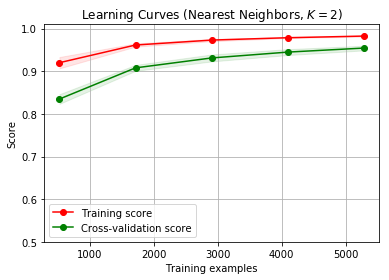
\includegraphics[width=\textwidth]{../figures/knn-results.png}
\end{figure}}

\only<3>{\begin{figure}
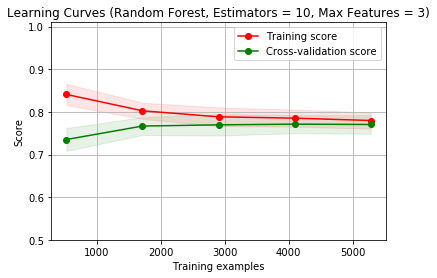
\includegraphics[width=\textwidth]{../figures/random-forest.png}
\end{figure}}

\only<4>{\begin{figure}
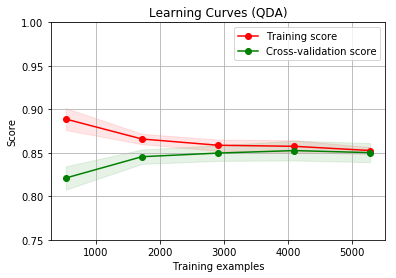
\includegraphics[width=\textwidth]{../figures/qda.png}
\end{figure}}

\end{columns}


\end{frame}

%-------------------------------------------------
\begin{frame}
\frametitle{Entrenamiento de clasificadores}

\begin{itemize}
\item Red utilizada es una red neuronal profunda con dos capas ocultas, la primera de ellas tiene 256 neuronas o nodos, mientras que la segunda capa posee 64 neuronas.

\item 20000 epoch, \textit{learning rate}  igual a $\alpha = 0.3$ . También se define un \textit{batch size} igual a 32.
\end{itemize}
\begin{columns}[t] 
\column{.5\textwidth} % Left column and width

\begin{figure}
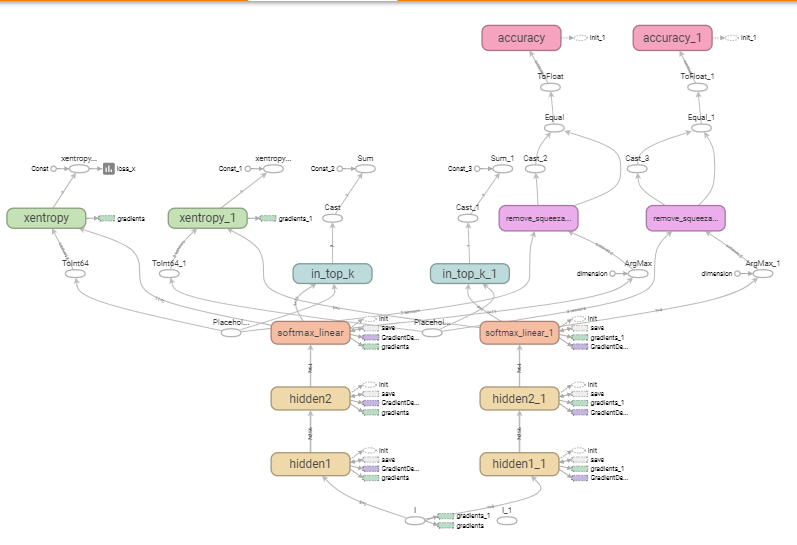
\includegraphics[width=\textwidth]{../figures/nn_estructura.png}
\end{figure}



\column{.5\textwidth} % Right column and width
\begin{figure}
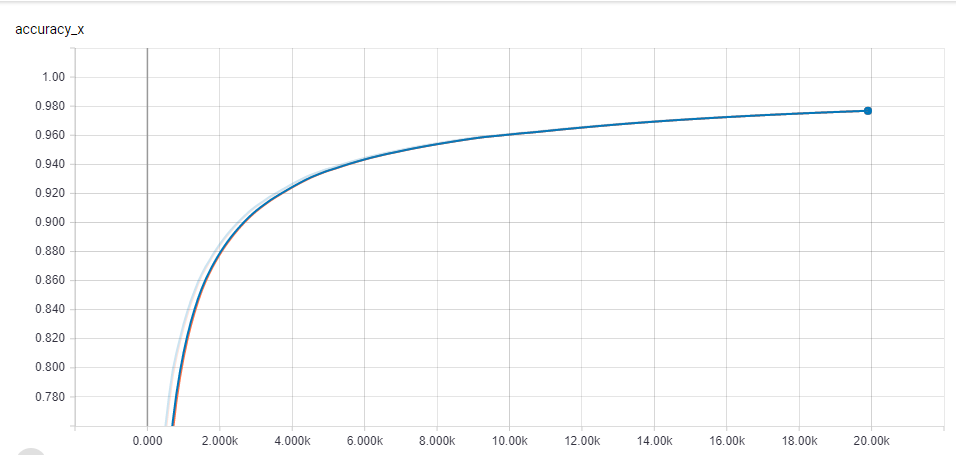
\includegraphics[width=\textwidth]{../figures/nn_plot.png}
\end{figure}

\end{columns}


\end{frame}


%-------------------------------------------------
\begin{frame}
\frametitle{Tabla de entrenamiento}

\begin{table}[ht!]
\centering
\resizebox{\textwidth}{!}{%
\begin{tabular}{|c|c|c|c|c|}
\hline
Algoritmo                     & Accuracy & Error medio X & Error medio Y & Error Absoluto \\ \hline
NN                            & 97.94\%  & 0.1579        & 0.0735        & 0.1741         \\ \hline
$SVM(RBF, C=1, \gamma = 4)$   & 96.81\%  & 0.2254        & 0.1018        & 0.2473         \\ \hline
$KNN(k = 2)$                  & 95.43\%  & 0.9842        & 0.1575        & 0.9967         \\ \hline
QDA                           & 85.25\%  & 5.1103        & 4.7175        & 6.9548         \\ \hline
$SVM(Lineal, C=1)$            & 78.75\%  & 9.3163        & 6.0387        & 11.1022        \\ \hline
Random Forest                 & 77.33\%  & 11.3430       & 3.1409        & 11.7698        \\ \hline
Naive Bayes                   & 71.73\%  & 12.2303       & 9.4836        & 15.4763        \\ \hline
Decision Tree( max depth = 5) & 57.91\%  & 57.8012       & 5.6412        & 58.0758        \\ \hline
Adaboost                      & 26.03\%  & 150.8848      & 6.5333        & 151.0261       \\ \hline
\end{tabular}
}
\end{table}


\end{frame}

%-------------------------------------------------
\begin{frame}
\frametitle{Entrenamiento utilizando PCA}

\begin{itemize}
\item Determinar número de componentes principales que deben ser utilizadas.
\pause
\item No existe un algoritmo que lo determine automáticamente.
\pause
\item Se proponen tres métodos para encontrar las componentes principales:

\begin{enumerate}[1]
\pause
	\item El primer método se basa en la información contextual presente en los valores propios.
	\pause
	\item Para el segundo método, es necesario establecer la suma acumulada porcentual de la varianza explicada.
	\pause
	\item Con respecto al tercer método, este se basa en seleccionar las primeras componentes principales según los resultados obtenidos en los clasificadores.
\end{enumerate}
\end{itemize}

\end{frame}

%-------------------------------------------------
\begin{frame}
\frametitle{Entrenamiento utilizando PCA}

\only<1>{\begin{columns}[t] % The "c" option specifies centered vertical alignment while the "t" option is used for top vertical alignment

\column{.5\textwidth} % Left column and width

\begin{figure}
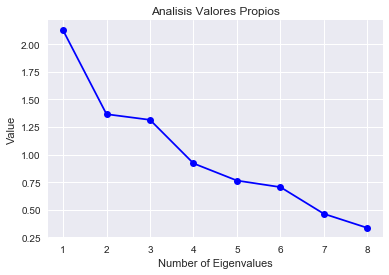
\includegraphics[width=\textwidth]{../figures/eigenvalues.png}
\end{figure}

\column{.5\textwidth} % Right column and width
\begin{figure}
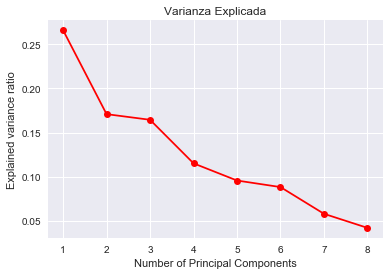
\includegraphics[width=\textwidth]{../figures/varianza_ratio.png}
\end{figure}
 % Right column and widt

\end{columns}}

\only<2>{\begin{figure}
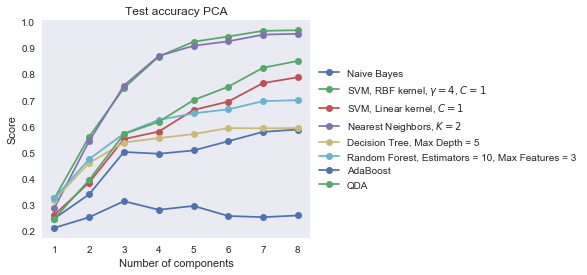
\includegraphics[width=\textwidth]{../figures/comparativa_clasificadores_pca.png}
\end{figure}}


\end{frame}

%-------------------------------------------------
\begin{frame}
\frametitle{Entrenamiento utilizando PCA}

\begin{table}[ht!]
\centering
\resizebox{\textwidth}{!}{%
\begin{tabular}{|c|c|c|c|c|}
\hline
Algoritmo                     & Accuracy & Error medio X & Error medio Y & Error Absoluto \\ \hline
NN                            & 93\%  & 1.8956        & 0.6589        & 2.0068         \\ \hline
$SVM(RBF, C=1, \gamma = 4)$   & 92.39\%  & 2.4581  & 0.7830        & 2.5797         \\ \hline
$KNN(k = 2)$                  & 90.83\%  & 2.1381 & 0.4872        & 2.1929         \\ \hline
QDA                           & 71.25\%  & 15.9418 & 9.3042        & 18.4583         \\ \hline
$SVM(Lineal, C=1)$            & 66.20\%  & 19.5878 & 10.4824        & 22.2162        \\ \hline
Random Forest                 & 64.15\%  & 21.3284 & 5.4472        & 22.0130       \\ \hline
Decision Tree( max depth = 5) & 56.96\%  & 33.5151       & 8.9163       & 34.6808        \\ \hline
Naive Bayes                   & 50.71\%  & 31.3406 & 10.0727        & 32.9194        \\ \hline
Adaboost                      & 32.20\%  & 73.9345 & 9.3042       & 74.5176       \\ \hline
\end{tabular}
}
\end{table}


\end{frame}


%-------------------------------------------------
\begin{frame}
\frametitle{Fase Online}

\begin{itemize}
\item No hay forma de determinar el error absoluto, producto de que para ello se debe proporcionar la posición real.

\pause
\item Lo que se propone para determinar los resultados son dos formas llamadas método estático y método dinámico.
\begin{enumerate}[1]
\pause
\item En el método estático lo que se hace es permanecer quieto en un determinado punto durante un tiempo predefinido. El tiempo utilizado en este caso corresponde a 15 minutos.

\pause
\item Para el caso del método dinámico, lo que se busca es abarcar la mayor cantidad de puntos posibles. En este caso se decide hacer una caminata a través de todos los 44 puntos.
\end{enumerate}
\end{itemize}


\end{frame}

%-------------------------------------------------
\begin{frame}
\frametitle{Fase Online}

\begin{columns}[t] % The "c" option specifies centered vertical alignment while the "t" option is used for top vertical alignment

\column{.3\textwidth} % Left column and width
\begin{figure}
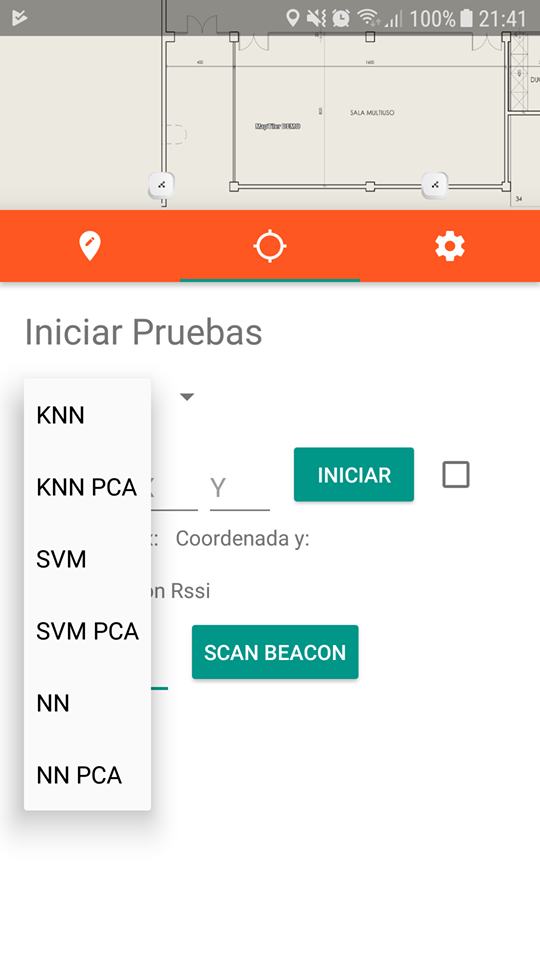
\includegraphics[width=\textwidth]{../figures/fase_online1.png}
\end{figure}

\column{.3\textwidth} % Right column and width
\begin{figure}
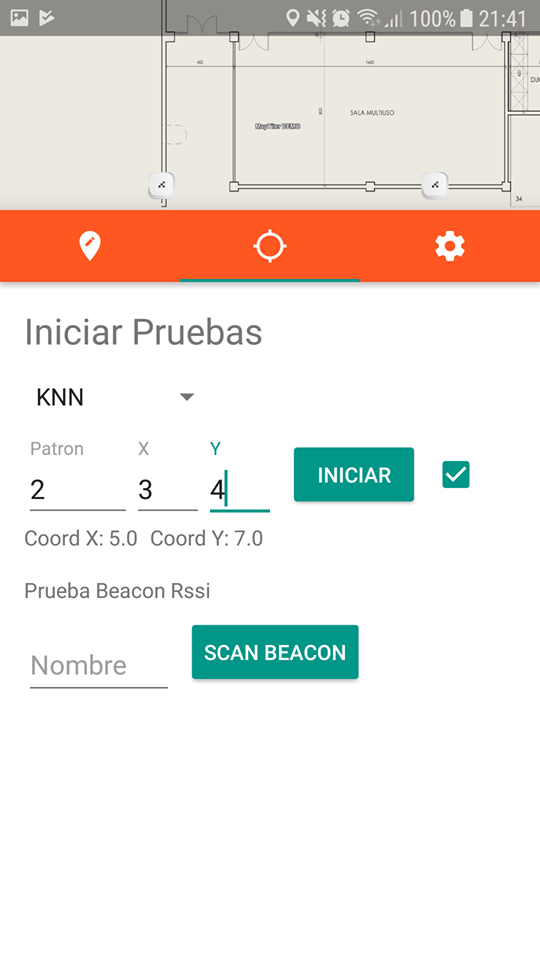
\includegraphics[width=\textwidth]{../figures/fase_online2.png}
\end{figure}

\column{.3\textwidth} % Right column and width
\begin{figure}
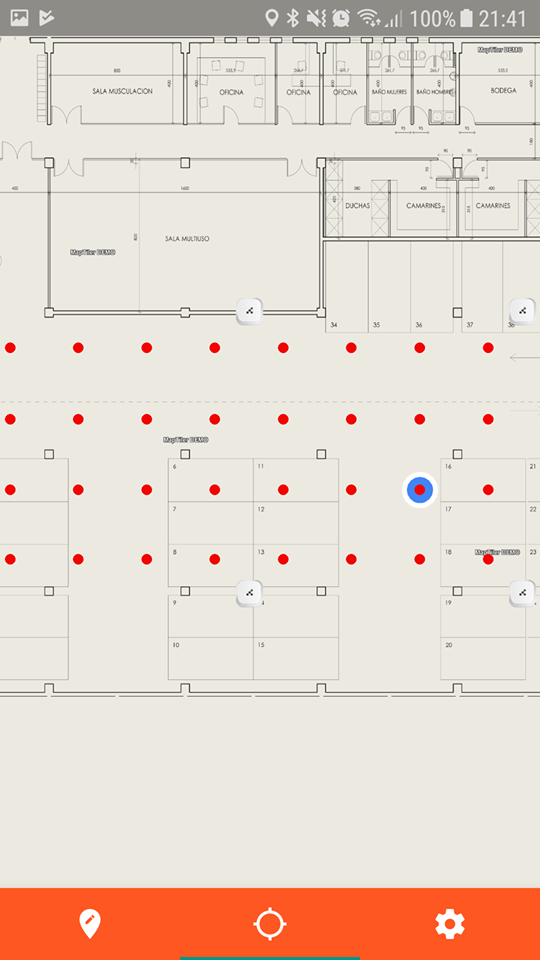
\includegraphics[width=\textwidth]{../figures/fase_online3.png}
\end{figure}

\end{columns}

\end{frame}

%-------------------------------------------------
\section{Resultados}
%-------------------------------------------------

\subsection{Métricas Obtenidas}
\begin{frame}
\frametitle{Errores medios método dinámico}

Método dinámico sin PCA

\begin{table}[ht!]
\centering
\resizebox{\textwidth}{!}{%
\begin{tabular}{|c|c|c|c|c|c|}
\hline
Clasificador & Error x & Error y & Varianza x & Varianza y & RMSE    \\ \hline
KNN          & 1.5858  & 4.6391  & 7.1970     & 2.1780     & 6.9323  \\ \hline
SVM          & 6.8207  & 2.8874  & 1.7243     & 0.5989     & 10.0323 \\ \hline
NN           & 4.3784  & 3.9113  & 13.0950    & 5.0712     & 8.2994  \\ \hline
\end{tabular}
}
\end{table}

Método dinámico con PCA
\begin{table}[!ht]
\centering
\resizebox{\textwidth}{!}{%
\begin{tabular}{|c|c|c|c|c|c|}
\hline
Clasificador & Error x & Error y & Varianza x & Varianza y & RMSE   \\ \hline
KNN PCA      & 2.0023  & 4.3983  & 7.5113     & 2.0696     & 6.6812 \\ \hline
SVM PCA      & 6.8948  & 2.4257  & 4.1134     & 2.0348     & 9.5668 \\ \hline
NN PCA       & 5.8874  & 4.4513  & 8.6088     & 3.2089     & 9.5188 \\ \hline
\end{tabular}
}
\end{table}


\end{frame}

%-------------------------------------------------
\begin{frame}
\frametitle{Errores medios método estático}

Método estático sin PCA

\begin{table}[!h]
\centering
\resizebox{\textwidth}{!}{%
\begin{tabular}{|c|c|c|c|c|c|}
\hline
Clasificador & Error x & Error y & Varianza x & Varianza y & RMSE   \\ \hline
KNN          & 3.2385  & 1.5417  & 3.3321     & 1.0940     & 5.0520 \\ \hline
SVM          & 5.2493  & 1.6986  & 2.0598     & 0.7594     & 7.0241 \\ \hline
NN           & 3.7300  & 2.1937  & 5.8885     & 0.7373     & 4.4857 \\ \hline
\end{tabular}
}
\end{table}

Método estático con PCA
\begin{table}[!h]
\centering
\resizebox{\textwidth}{!}{%
\begin{tabular}{|c|c|c|c|c|c|}
\hline
Clasificador & Error x & Error y & Varianza x & Varianza y & RMSE   \\ \hline
KNN PCA      & 2.9892  & 1.4475  & 3.1487     & 1.6391     & 5.0340 \\ \hline
SVM PCA      & 3.2313  & 1.4905  & 3.0630     & 1.7817     & 5.1757 \\ \hline
NN PCA       & 1.5578  & 1.7488  & 3.8045    & 2.6885     & 3.9341 \\ \hline
\end{tabular}
}
\end{table}

\end{frame}
%-------------------------------------------------
\begin{frame}
\frametitle{Cumulative distribution function Dinámico}

$$
F_{X} (x) = P(X \le x)
$$

\begin{columns}[t] % The "c" option specifies centered vertical alignment while the "t" option is used for top vertical alignment

\column{.5\textwidth} % Left column and width

\only<1>{\begin{figure}
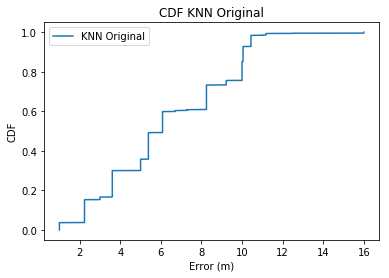
\includegraphics[width=\textwidth]{../figures/cdf-knn-dinamico.png}
\end{figure}}

\only<2>{\begin{figure}
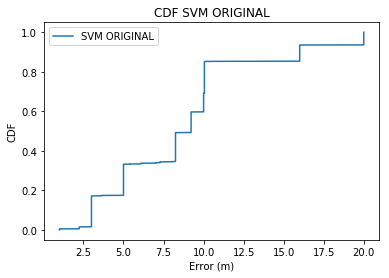
\includegraphics[width=\textwidth]{../figures/cdf-svm-dinamico.png}
\end{figure}}

\only<3>{\begin{figure}
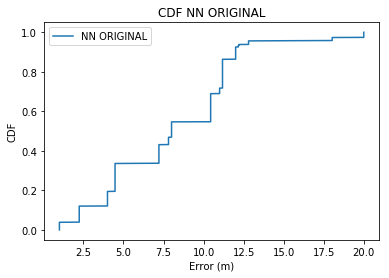
\includegraphics[width=\textwidth]{../figures/cdf-nn-dinamico.png}
\end{figure}}

\column{.5\textwidth} % Right column and width
\only<1>{\begin{figure}
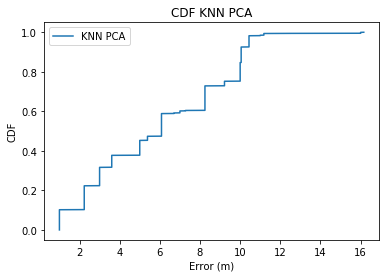
\includegraphics[width=\textwidth]{../figures/cdf-knnPCA-dinamico.png}
\end{figure}}

\only<2>{\begin{figure}
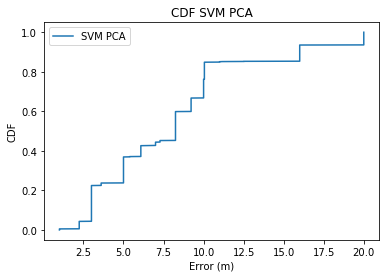
\includegraphics[width=\textwidth]{../figures/cdf-svmPCA-dinamico.png}
\end{figure}}

\only<3>{\begin{figure}
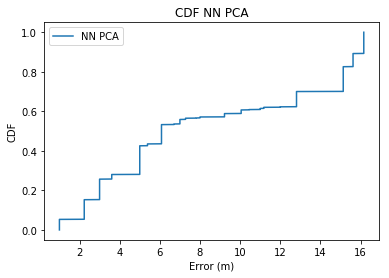
\includegraphics[width=\textwidth]{../figures/cdf-nnPCA-dinamico.png}
\end{figure}}

\end{columns}

\only<4>{\begin{table}[!h]
\centering
\resizebox{\textwidth}{!}{%
\begin{tabular}{|c|c|c|c|}
\hline
Clasificador & Sin PCA & Con PCA & Mejora     \\ \hline
KNN          & 16.576  & 16.1554 & 2.5374 \%  \\ \hline
SVM          & 20.8962 & 19.3874 & 7.2204 \%  \\ \hline
NN           & 20.5677 & 16.1554 & 21.4525 \% \\ \hline
\end{tabular}
}
\end{table}}

\end{frame}

%-------------------------------------------------
\begin{frame}
\frametitle{Cumulative distribution function Estático}

$$
F_{X} (x) = P(X \le x)
$$

\begin{columns}[t] % The "c" option specifies centered vertical alignment while the "t" option is used for top vertical alignment

\column{.5\textwidth} % Left column and width

\only<1>{\begin{figure}
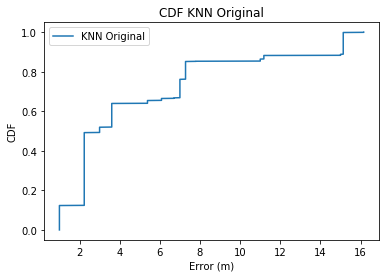
\includegraphics[width=\textwidth]{../figures/cdf-knn-estatico.png}
\end{figure}}

\only<2>{\begin{figure}
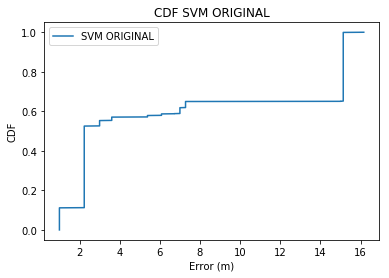
\includegraphics[width=\textwidth]{../figures/cdf-svm-estatico.png}
\end{figure}}

\only<3>{\begin{figure}
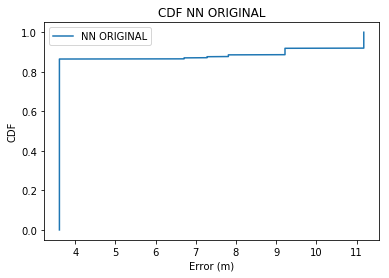
\includegraphics[width=\textwidth]{../figures/cdf-nn-estatico.png}
\end{figure}}

\column{.5\textwidth} % Right column and width
\only<1>{\begin{figure}
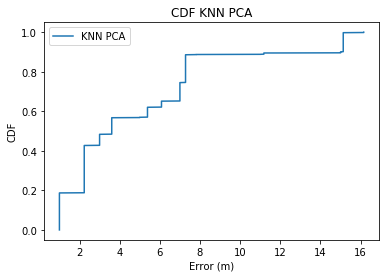
\includegraphics[width=\textwidth]{../figures/cdf-knnPCA-estatico.png}
\end{figure}}

\only<2>{\begin{figure}
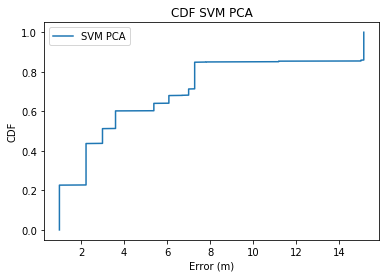
\includegraphics[width=\textwidth]{../figures/cdf-svmPCA-estatico.png}
\end{figure}}

\only<3>{\begin{figure}
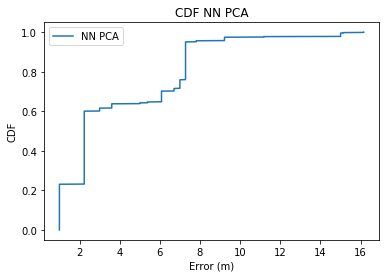
\includegraphics[width=\textwidth]{../figures/cdf-nnPCA-estatico.png}
\end{figure}}

\end{columns}

\only<4>{\begin{table}[!h]
\centering
\resizebox{\textwidth}{!}{%
\begin{tabular}{|c|c|c|c|}
\hline
Clasificador & Sin PCA  & Con PCA & Cambio    \\ \hline
KNN          & 16.1554  & 16.1554 & 0 \%      \\ \hline
SVM          & 16.1554  & 15.1327 & 6.33 \%   \\ \hline
NN           & 11.18033 & 16.1554 & -44.49 \% \\ \hline
\end{tabular}
}
\end{table}}

\end{frame}

%-------------------------------------------------
\begin{frame}
\frametitle{Análisis de distribución}

\begin{figure}
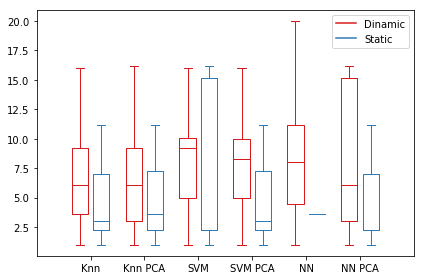
\includegraphics[width=\textwidth]{../figures/boxplot.png}
\end{figure}

\end{frame}

%-------------------------------------------------
\begin{frame}
\frametitle{Análisis tiempos de ejecución}

Resultados en términos de milisegundos con su respectiva mejora.

\begin{table}[ht!]
\centering
\resizebox{\textwidth}{!}{%
\begin{tabular}{|c|c|c|c|}
\hline
\textbf{Clasificador} & \textbf{Sin PCA} & \textbf{Con PCA} & \textbf{Incremento} \\ \hline
KNN                   & 64.9642          & 59.6786          & 8.1361\%            \\ \hline
SVM                   & 54.5985          & 25.6085          & 53.0966\%           \\ \hline
NN                    & 0.7610           & 0.5777           & 24.0867\%           \\ \hline
\end{tabular}
}
\end{table}

\end{frame}

%-------------------------------------------------
\subsection{Análisis de resultados}
\begin{frame}
\frametitle{Análisis de resultados}

\begin{itemize}

\item Resultados estáticos son mucho mejores que los resultados dinámicos, sin embargo, el escenario de que el usuario este estático en un punto es menos realista.
\pause

\item Los mejores valores de error medio son obtenidos por KNN y NN, en ambos métodos (estático y dinámico).
\pause

\item KNN es mucho menos disperso en ambos métodos y sus errores están más centrados en valores bajos, mientras NN presenta mucho mayor dispersión en el método dinámico, pero casi nada en el método estático, sobre todo al no utilizar PCA.
\pause

\item Mejor algoritmo es redes neuronales, a pesar de su distribución, mantiene valores bajos de error y tiempos de procesamiento.

\end{itemize}



\end{frame}

%-------------------------------------------------
\section{Conclusiones}
%-------------------------------------------------

%-------------------------------------------------
\begin{frame}
\frametitle{Conclusiones}

\begin{itemize}

\item Las señales Bluetooth se ven afectadas profundamente por cualquier objeto que se interponga, inclusive el cuerpo humano.
\pause

\item Los datos recolectados presentan estructuras no lineales, y correlaciones lineales localmente. Mejores algoritmos son aquellos capaces de reconocer estas estructuras.
\pause

\item Mejor algoritmo es Neural Network, considerando su error, tiempo de computo, a pesar de tener mayor dispersión en los datos.

\pause

\item Se debe utilizar PCA adecuadamente.

\pause

\item Técnicas de máquinas de aprendizaje, pueden reducir el error a unos pocos metros, lo cual es alto si se considera un posicionamiento en tiempo real. 

\end{itemize}

\end{frame}

%-------------------------------------------------
\begin{frame}
\frametitle{Conclusiones}

\begin{itemize}

\item Se requiere mayor en investigación en cuanto a determinar densidad de Beacons, tamaño de grilla, y otros factores asociados a la implementación.
\pause

\item Recolección de Fingerprints es un proceso lento, y debe ser mejorado. Se puede utilizar aprendizaje no supervisado.
\pause

\item Las máquinas de aprendizaje en conjunto con las señales Bluetooth Low Energy pueden ser un punto de partida para la fusión de sensores.

\pause
\item El mayor problema del posicionamiento en interiores es lograr un modelo estándar.

\end{itemize}

\end{frame}

%------------------------------------------------
\begin{frame}
\Huge{\centerline{Gracias por su atención}}
\end{frame}

%------------------------------------------------

\end{document}

